% Meeting Oliver x Dr. Soleimani x Nishioka, 2026-10-20 (moved from 19 Oct) (coupling ideas)
% Copy of slides_1005.tex with one added frame: growth from the living biomass, first results
% Build: .\build_slides.ps1   (pdflatex, twice)
% Speaker script (EN + JA, one section per slide): speaker_notes_1005.tex
% CONSTRAINT: keep total page count <= 30 (19 Oct deck, the user, 15 Oct). Check the built PDF's page count
% before adding a frame; trim an existing frame rather than tacking more on.
% Wording: no internal labels (run names, switch numbers) -- say what a run
% does, not what it was called while building it.
\documentclass[aspectratio=169,11pt]{beamer}
\usetheme{Madrid}
\usecolortheme{seahorse}
\usepackage{booktabs}
\usepackage{array}
\usepackage{amsmath,amssymb}
\usepackage{bm}
\usepackage{xcolor}
\usepackage{graphicx}
\usepackage{tikz}
\usetikzlibrary{arrows.meta,positioning}

\definecolor{c3}{RGB}{30,80,160}
\definecolor{warn}{RGB}{200,30,30}
\tikzset{fbox/.style={draw,rounded corners,align=center,font=\footnotesize,minimum height=0.95cm,text width=#1},
  fbox/.default=2.3cm,
  used/.style={fbox,fill=gray!15},
  mine/.style={fbox,fill=c3!18,draw=c3},
  arr/.style={-{Latex[length=2mm]},thick}}
\setbeamercolor{frametitle}{bg=c3, fg=white}
\setbeamertemplate{navigation symbols}{}

\title{Master's Thesis: Status and Plan}
\subtitle{Biofilm growth coupled into the IKM FEM element, following Klempt et al.}
\author[Keisuke Nishioka]{Keisuke Nishioka}
\institute[IKM, LUH]{%
\small Institute of Continuum Mechanics (IKM), Leibniz Universit\"at Hannover\\
\small Keio University}
\date{20 October 2026}

\begin{document}
\maketitle


% --------------------------------------------------------
\begin{frame}{Since the last meeting: the scope of the FEM part is fixed}
\centering\small\renewcommand{\arraystretch}{1.35}
\begin{tabular}{@{}>{\raggedright}p{0.17\linewidth}>{\raggedright}p{0.27\linewidth}>{\raggedright}p{0.22\linewidth}>{\raggedright\arraybackslash}p{0.24\linewidth}@{}}
\toprule
 & content & reference & coupling\\
\midrule
\multicolumn{4}{@{}l}{\textcolor{c3}{\textbf{thesis (LUH)}}}\\
one species & growth law, Eq.\ 36 & Klempt et al.\ 2024 & field $\to$ growth\\
two species & composition from the point model & Klempt et al.\ 2026 & field $\to$ composition (one-way)\\
\midrule
\multicolumn{4}{@{}l}{\textcolor{black!60}{\textbf{continuation (Keio)}}}\\
five species & calibrated point model; first runs in Appendix G & none yet & two-way: composition and stress act back\\
\bottomrule
\end{tabular}

\vspace{10pt}
One and two species can be checked against published examples; five species have no reference yet.
\end{frame}

% --------------------------------------------------------
\begin{frame}{Verification, step by step}
\centering
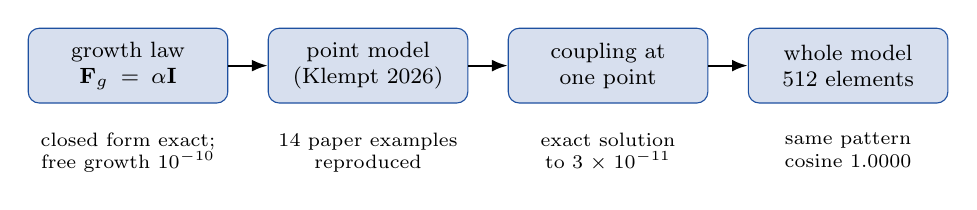
\begin{tikzpicture}[ node distance=0.35cm and 0.5cm]
\node[mine] (a) {growth law\\ $\mathbf F_g=\alpha\mathbf I$};
\node[mine,right=of a] (b) {point model\\ (Klempt 2026)};
\node[mine,right=of b] (c) {coupling at\\ one point};
\node[mine,right=of c] (d) {whole model\\ 512 elements};
\draw[arr] (a)--(b); \draw[arr] (b)--(c); \draw[arr] (c)--(d);
\node[below=0.25cm of a,font=\scriptsize,text width=2.3cm,align=center] {closed form exact;\\ free growth $10^{-10}$};
\node[below=0.25cm of b,font=\scriptsize,text width=2.3cm,align=center] {14 paper examples\\ reproduced};
\node[below=0.25cm of c,font=\scriptsize,text width=2.3cm,align=center] {exact solution\\ to $3\times10^{-11}$};
\node[below=0.25cm of d,font=\scriptsize,text width=2.3cm,align=center] {same pattern\\ cosine 1.0000};
\end{tikzpicture}

\vspace{14pt}
\small Each step is checked before the next one builds on it.
\begin{itemize}\footnotesize
  \item point model: two misprints in Klempt et al.\ 2026 identified (no $+\gamma$ in Eq.\ 17, no $\tfrac12$ in Eq.\ 19)
  \item same point model in Fritsch et al.\ 2025: their figures reproduced within 0.013
\end{itemize}
\end{frame}

% --------------------------------------------------------
\begin{frame}{The coupling: what the element does and what is added}
\centering
\small The element solves the biofilm field of Klempt et al.\ 2024 (Eq.\ 34):
\[
\dot\phi-\beta\,\Delta\phi-k_\alpha\,\alpha
+|\nabla\phi|\,r\,\frac{c}{k+c}\,\mathbf n_\phi\!\cdot\mathbf n_c=0
\]
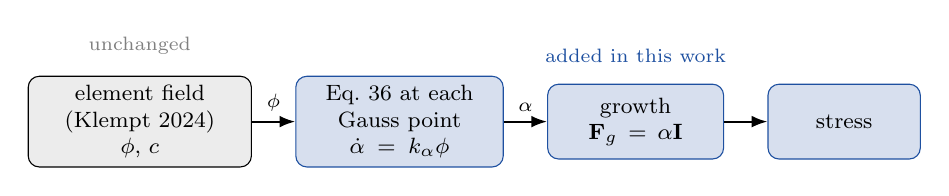
\begin{tikzpicture}[ node distance=0.45cm and 0.55cm]
\node[used,fbox=2.6cm] (f) {element field\\ (Klempt 2024)\\ $\phi$, $c$};
\node[mine,fbox=2.4cm,right=of f] (e) {Eq.\ 36 at each\\ Gauss point\\ $\dot\alpha=k_\alpha\phi$};
\node[mine,fbox=2.0cm,right=of e] (g) {growth\\ $\mathbf F_g=\alpha\mathbf I$};
\node[mine,fbox=1.7cm,right=of g] (s) {stress};
\draw[arr] (f)--node[above,font=\scriptsize]{$\phi$}(e);
\draw[arr] (e)--node[above,font=\scriptsize]{$\alpha$}(g);
\draw[arr] (g)--(s);
\node[above=0.15cm of f,font=\scriptsize,text=gray] {unchanged};
\node[above=0.15cm of g,font=\scriptsize,text=c3] {added in this work};
\end{tikzpicture}

\vspace{12pt}
\footnotesize Klempt 2024 Table 2: $k_\alpha=10^{-3}$, $E=10$ Pa, $\nu=0.49$.
$\beta,r,k,d,g$: the framework's example input, not from the paper.
\end{frame}

% --------------------------------------------------------
\begin{frame}{Model and boundary conditions}
\vspace{-6pt}
\begin{center}
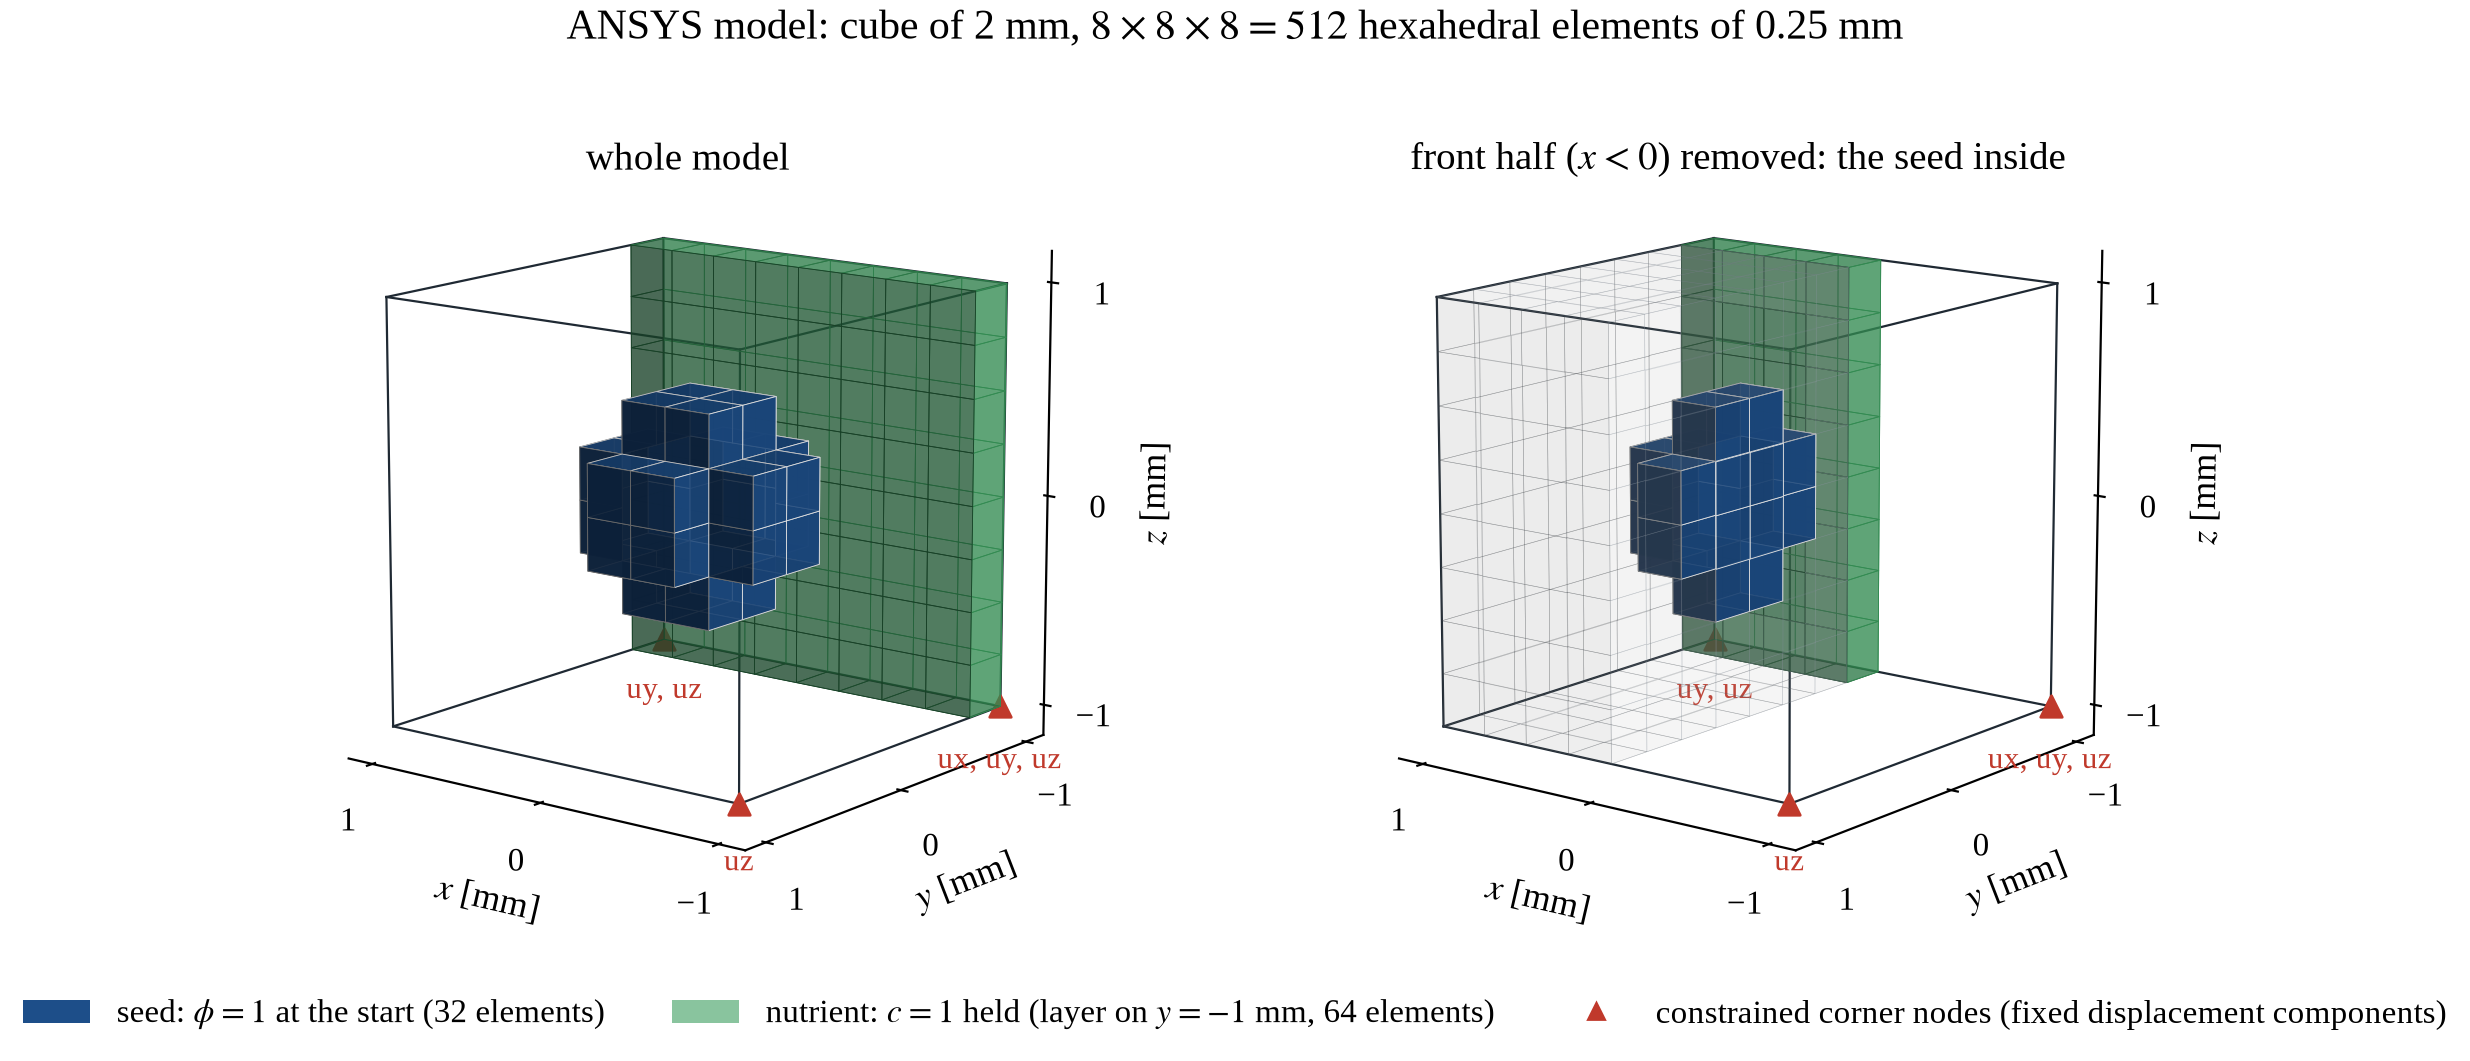
\includegraphics[width=\linewidth,height=0.5\textheight,keepaspectratio]{assets/fig_model_setup.png}
\end{center}
\vspace{-6pt}
\footnotesize
\begin{itemize}
  \item 2 mm cube, 512 elements; only rigid-body motion fixed
  \item nutrient $c=1$ on the face $y=-1$ mm; seed of 32 elements with $\phi=1$
  \item uniform growth is stress free; stress comes from differences in growth
  \item used for Checks 1--3 and the two-species runs (ANSYS); the Klempt 2024
        reproduction uses the paper's 20\,$\mu$m cube (Python)
\end{itemize}
\end{frame}


% --------------------------------------------------------
\begin{frame}{What I implemented}
\centering
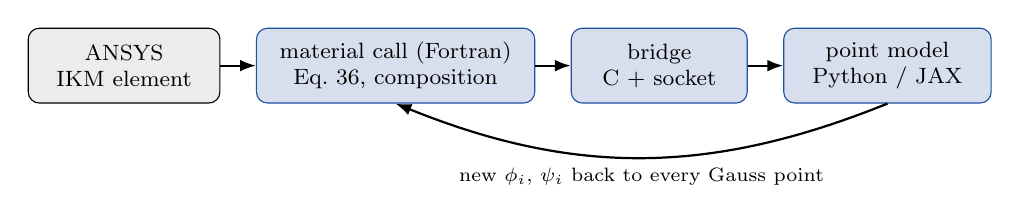
\begin{tikzpicture}[ node distance=0.5cm and 0.45cm]
\node[used,fbox=2.2cm] (a) {ANSYS\\ IKM element};
\node[mine,fbox=3.3cm,right=of a] (b) {material call (Fortran)\\ Eq.\ 36, composition};
\node[mine,fbox=2.0cm,right=of b] (c) {bridge\\ C + socket};
\node[mine,fbox=2.4cm,right=of c] (d) {point model\\ Python / JAX};
\draw[arr] (a)--(b); \draw[arr] (b)--(c); \draw[arr] (c)--(d);
\draw[arr] (d.south) to[bend left=22] node[below,font=\scriptsize]{new $\phi_i$, $\psi_i$ back to every Gauss point} (b.south);
\end{tikzpicture}

\vspace{10pt}
\begin{tabular}{@{}ll@{}}
\textbf{speed} & single-element run 357\,s $\to$ \textbf{5.6\,s}\\
\textbf{check} & every ANSYS call replayed in Python, difference 0\\
\end{tabular}

\vspace{6pt}
\begin{columns}[T]
\begin{column}{0.42\textwidth}\footnotesize
\textcolor{gray}{\textbf{used as it is}}
\begin{itemize}
  \item IKM element: field, stiffness
  \item point-model equations (Klempt et al.\ 2026)
\end{itemize}
\end{column}
\begin{column}{0.56\textwidth}\footnotesize
\textcolor{c3}{\textbf{written in this work}}
\begin{itemize}
  \item Eq.\ 36 and the composition step in the material call
  \item Fortran $\to$ Python bridge, sub-stepping
  \item point-model solver (JAX): all 14 paper examples
  \item checks: closed form in ANSYS, call replay, about 440 tests
\end{itemize}
\end{column}
\end{columns}
\end{frame}

% --------------------------------------------------------
\begin{frame}{Second version: the point model in Fortran}
\centering
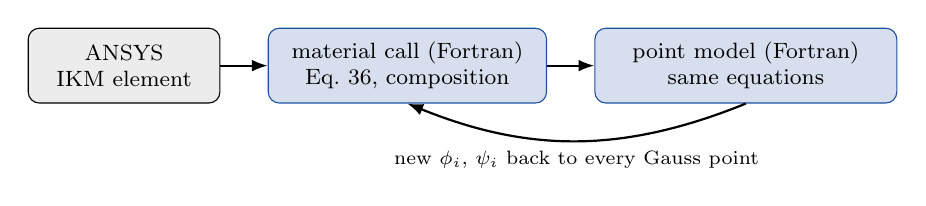
\begin{tikzpicture}[ node distance=0.5cm and 0.6cm]
\node[used,fbox=2.2cm] (a) {ANSYS\\ IKM element};
\node[mine,fbox=3.3cm,right=of a] (b) {material call (Fortran)\\ Eq.\ 36, composition};
\node[mine,fbox=3.6cm,right=of b] (d) {point model (Fortran)\\ same equations};
\draw[arr] (a)--(b); \draw[arr] (b)--(d);
\draw[arr] (d.south) to[bend left=22] node[below,font=\scriptsize]{new $\phi_i$, $\psi_i$ back to every Gauss point} (b.south);
\end{tikzpicture}

\vspace{8pt}
\small
\begin{itemize}
  \item replaces the bridge and the Python process; the material call is unchanged
  \item per sub-step: Newton on the $12$ unknowns $\phi_1..\phi_5,\ \phi_0,\ \psi_1..\psi_5,\ \gamma$
        ($6$ iterations), exact Jacobian written out, LU with pivoting
\end{itemize}

\vspace{4pt}
\footnotesize
\begin{tabular}{@{}ll@{}}
\toprule
\textbf{check} & \textbf{result}\\
\midrule
against the Python solver ($16$ states, $4$ cases) & largest relative difference $8\times10^{-15}$\\
ANSYS, $8^3$, two species, one week & stress, nutrient identical; point model $\le1.6\times10^{-12}$\\
run time, same model & $156$\,s $\to$ \textbf{36\,s}\\
\bottomrule
\end{tabular}

\vspace{6pt}
\footnotesize\textcolor{gray}{No server or port: one executable, so runs on a cluster or in parallel need no extra process.}
\end{frame}


% --------------------------------------------------------
\begin{frame}{Checks 1 and 2: exact solution and whole model}
\begin{columns}[T]
\begin{column}{0.5\textwidth}
\centering\small\textbf{1. Exact solution}\\
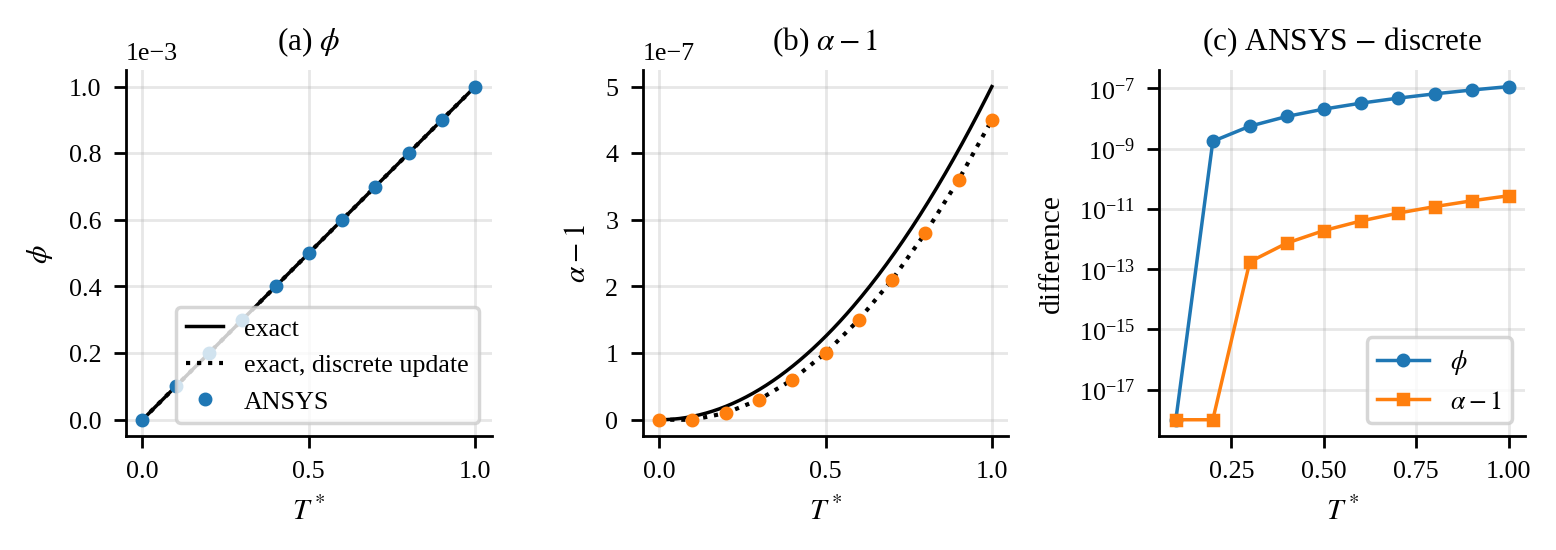
\includegraphics[width=\linewidth,height=0.5\textheight,keepaspectratio]{assets/fig1005_exact.png}\\
$\alpha$ matches to $3\times10^{-11}$
\end{column}
\begin{column}{0.48\textwidth}
\centering\small\textbf{2. Whole model, 512 elements}\\
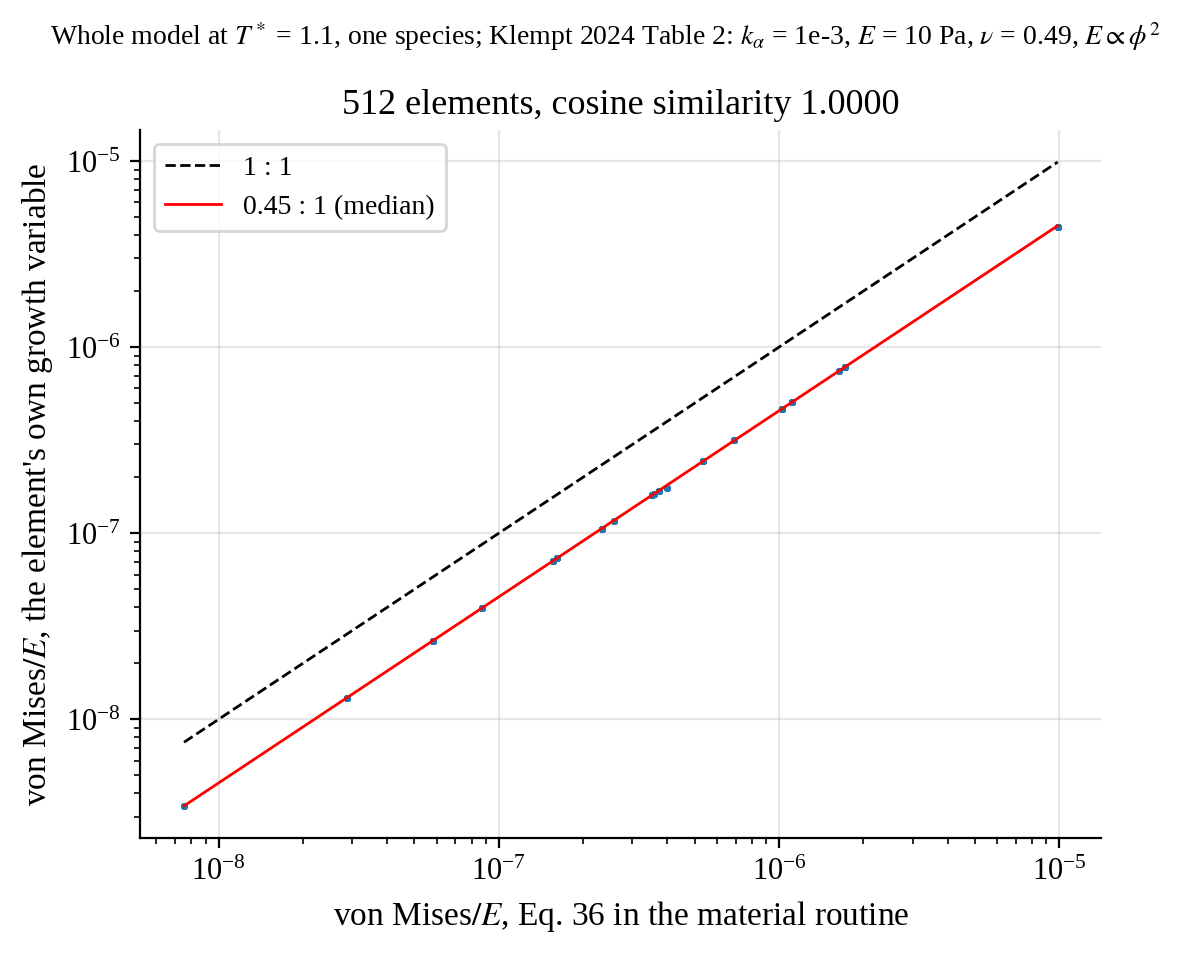
\includegraphics[width=\linewidth,height=0.5\textheight,keepaspectratio]{assets/fig1005_whole_model.png}\\
same pattern (cosine 1.0000); factor $0.455=\tfrac12\cdot\tfrac{10}{11}$
\end{column}
\end{columns}
\end{frame}

% --------------------------------------------------------
\begin{frame}{Check 3: the seeded element and its neighbours}
\vspace{-4pt}
\begin{center}
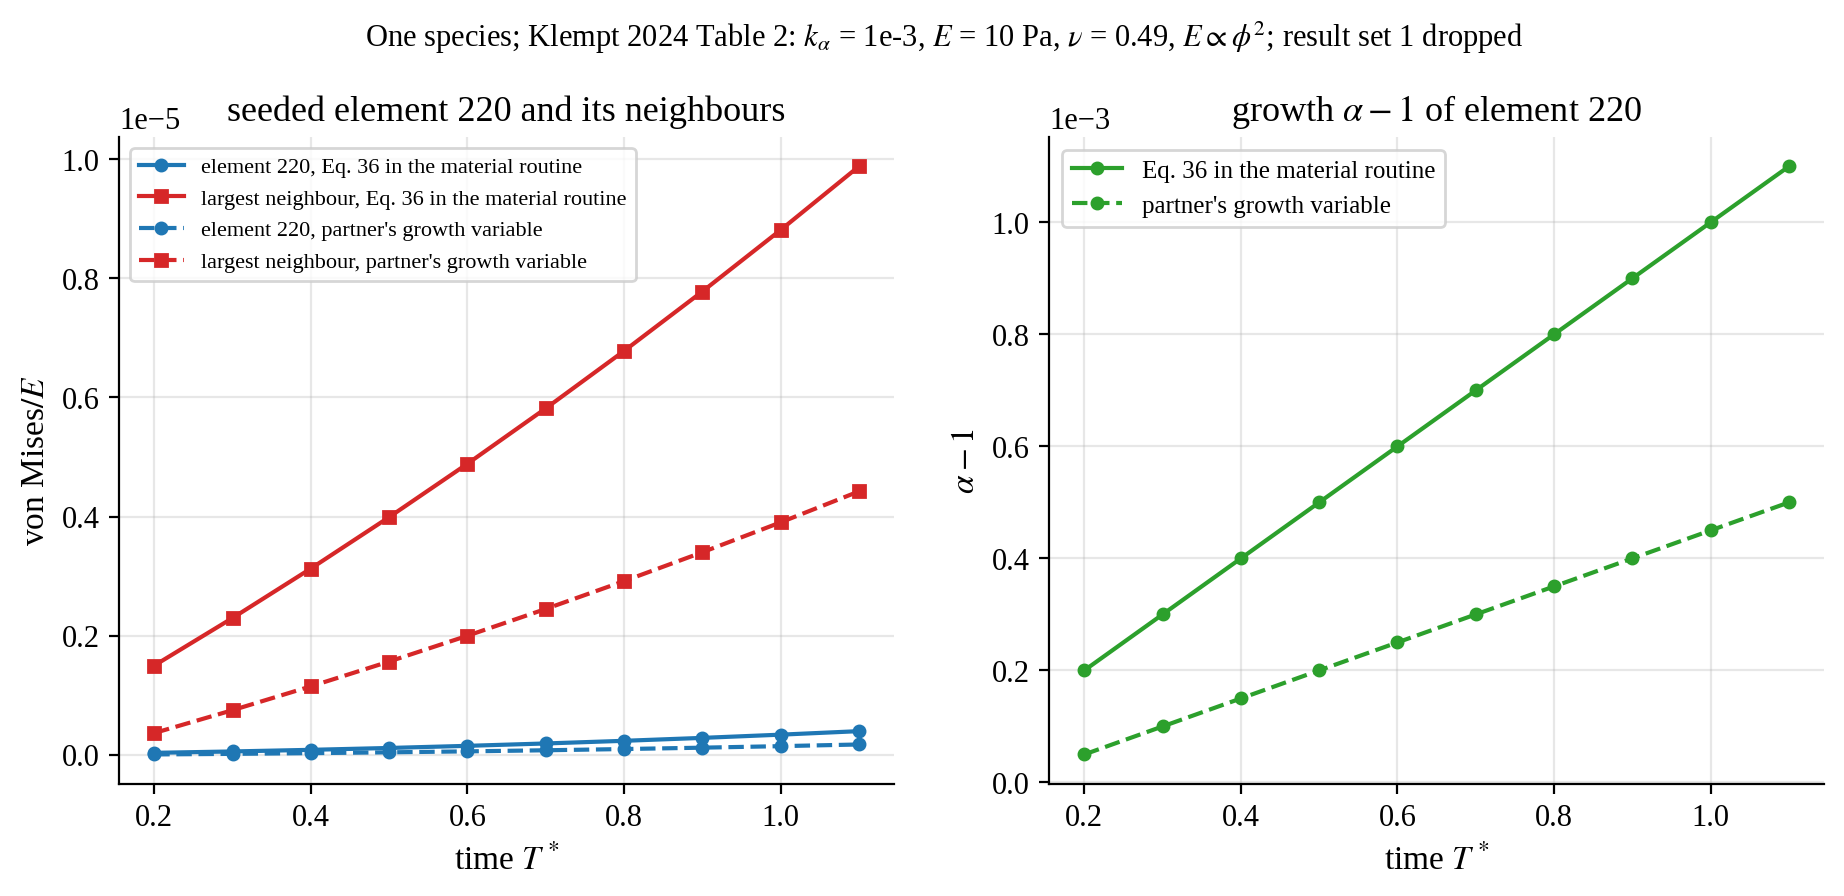
\includegraphics[width=\linewidth,height=0.58\textheight,keepaspectratio]{assets/fig1005_element220.png}
\end{center}
\vspace{-6pt}
\small
\begin{itemize}
  \item $\alpha-1=1.1\times10^{-3}=k_\alpha\phi t$, as Eq.\ 36 says
  \item seed compressed; neighbours carry about 25$\times$ its von Mises stress
  \item von Mises$/E\le10^{-5}$: slow growth (stresses scale with $E$)
\end{itemize}
\end{frame}

% --------------------------------------------------------
\begin{frame}{Four things found along the way (partner element)}
\centering\footnotesize\renewcommand{\arraystretch}{1.35}
\begin{tabular}{@{}c>{\raggedright}p{0.3\linewidth}>{\raggedright}p{0.3\linewidth}>{\raggedright\arraybackslash}p{0.28\linewidth}@{}}
\toprule
 & what I found & effect & what I did\\
\midrule
1 & growth variable is the mean of both species fields & growth halved with one species (unused field stays at its start value) & asked Oliver whether intended\\
2 & start values must satisfy $\phi_1+\phi_2\le1$ & example input starts both at 1 & one species: second field starts at 0\\
3 & first result set not in equilibrium & zero stress while the element sets up its operators & first result set excluded\\
4 & front-growth term inactive (reading slip); $|\Delta\phi|$ where Eq.\ 34 has $|\nabla\phi|$ & seed does not spread & corrected in a test copy: then $\phi$ exceeds 1\\
\bottomrule
\end{tabular}

\vspace{10pt}

\begin{tikzpicture}
\node[draw=c3,fill=c3!8,rounded corners,font=\small,inner sep=5pt] {Checks 1--3 do not depend on these four points.};
\end{tikzpicture}
\end{frame}

% --------------------------------------------------------
\begin{frame}{Two species: composition from the point model (Klempt et al.\ 2026)}
\vspace{-4pt}
\begin{center}
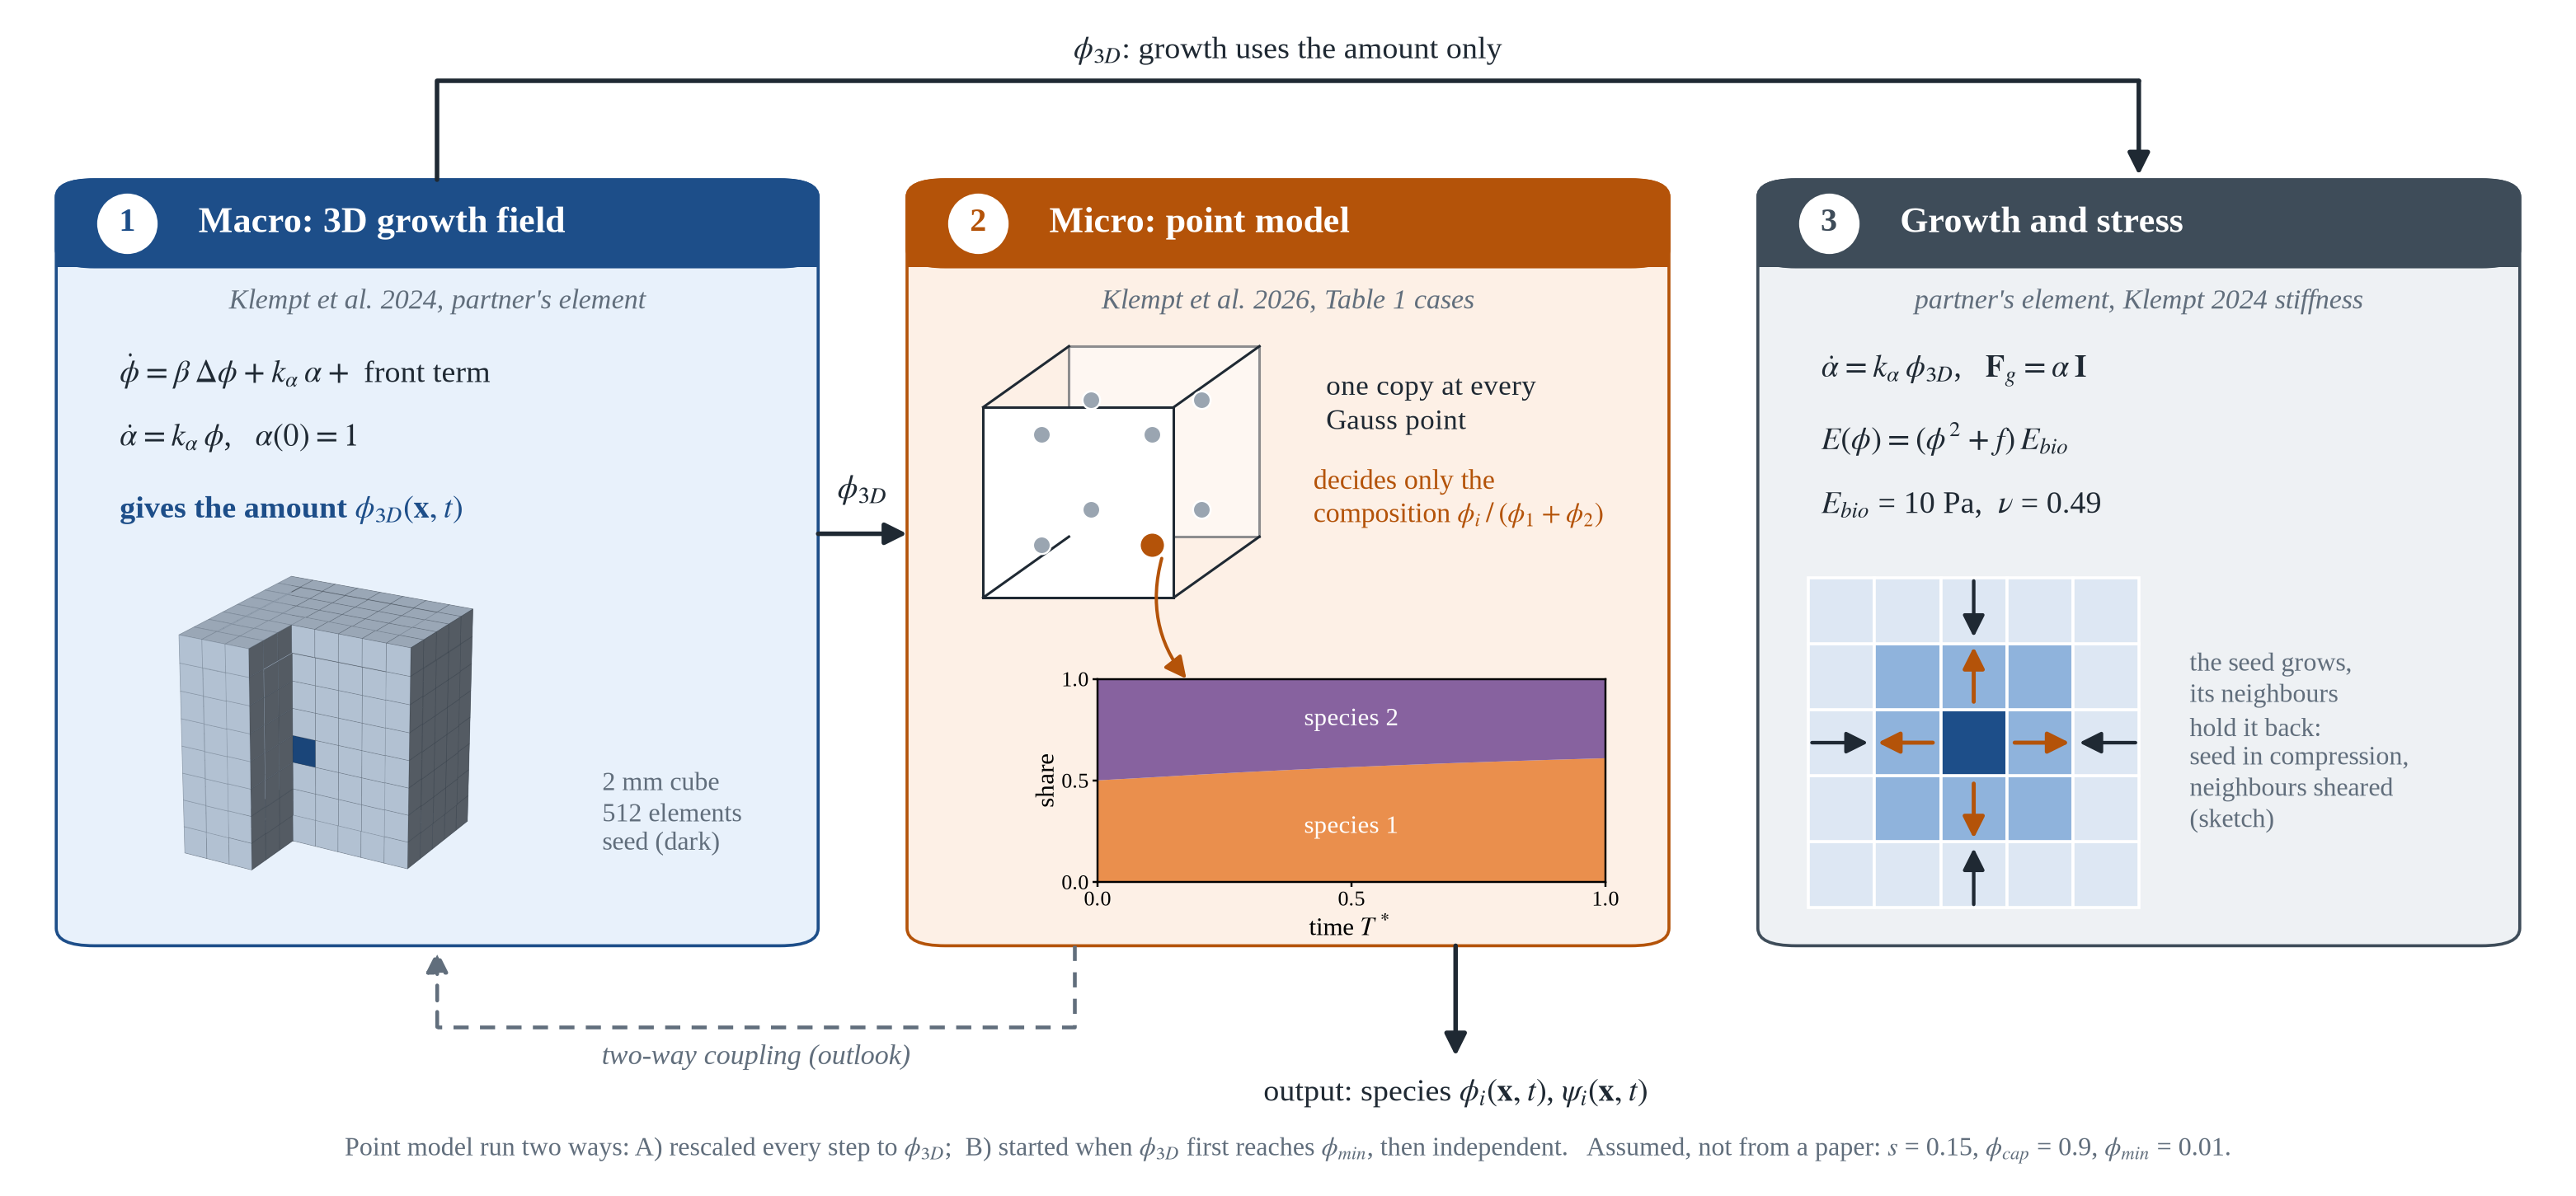
\includegraphics[width=\linewidth,height=0.66\textheight,keepaspectratio]{assets/fig_coupling_schematic.png}
\end{center}
\vspace{-6pt}
\small
\begin{itemize}
  \item the field sets the \textbf{amount}, the point model the \textbf{composition}
  \item one-way: the composition does not act on the stress
\end{itemize}
\end{frame}

% --------------------------------------------------------
\begin{frame}{Two species: results in the packed seed (ANSYS, $T^*=1$)}
\centering
\begin{tabular}{@{}llll@{}}
\toprule
case (Klempt et al.\ 2026) & paper & coupled, $\phi_{\rm cap}=0.9$ & $\phi_{\rm cap}=0.85$ / $0.95$\\
\midrule
3: coexistence & $0.60$ & $0.667$ & $0.668$ / $0.664$\\
6: one species wins & $\approx0$ ($\psi_1=0.05$) & $0.021$ ($\psi_1=0.048$) & --\\
\bottomrule
\end{tabular}\\[4pt]
\footnotesize share $\phi_1/(\phi_1+\phi_2)$; paper: point model alone; parameters $c^*=100$, $\alpha^*=10$
\vspace{10pt}
\begin{itemize}\small
  \item same type of outcome; the ratio shifts because the field sets the amount
  \item converged in the coupling time step
\end{itemize}
\end{frame}

% --------------------------------------------------------
\begin{frame}{Added since 5 October: growth from the living biomass}
\vspace{-6pt}
\begin{center}
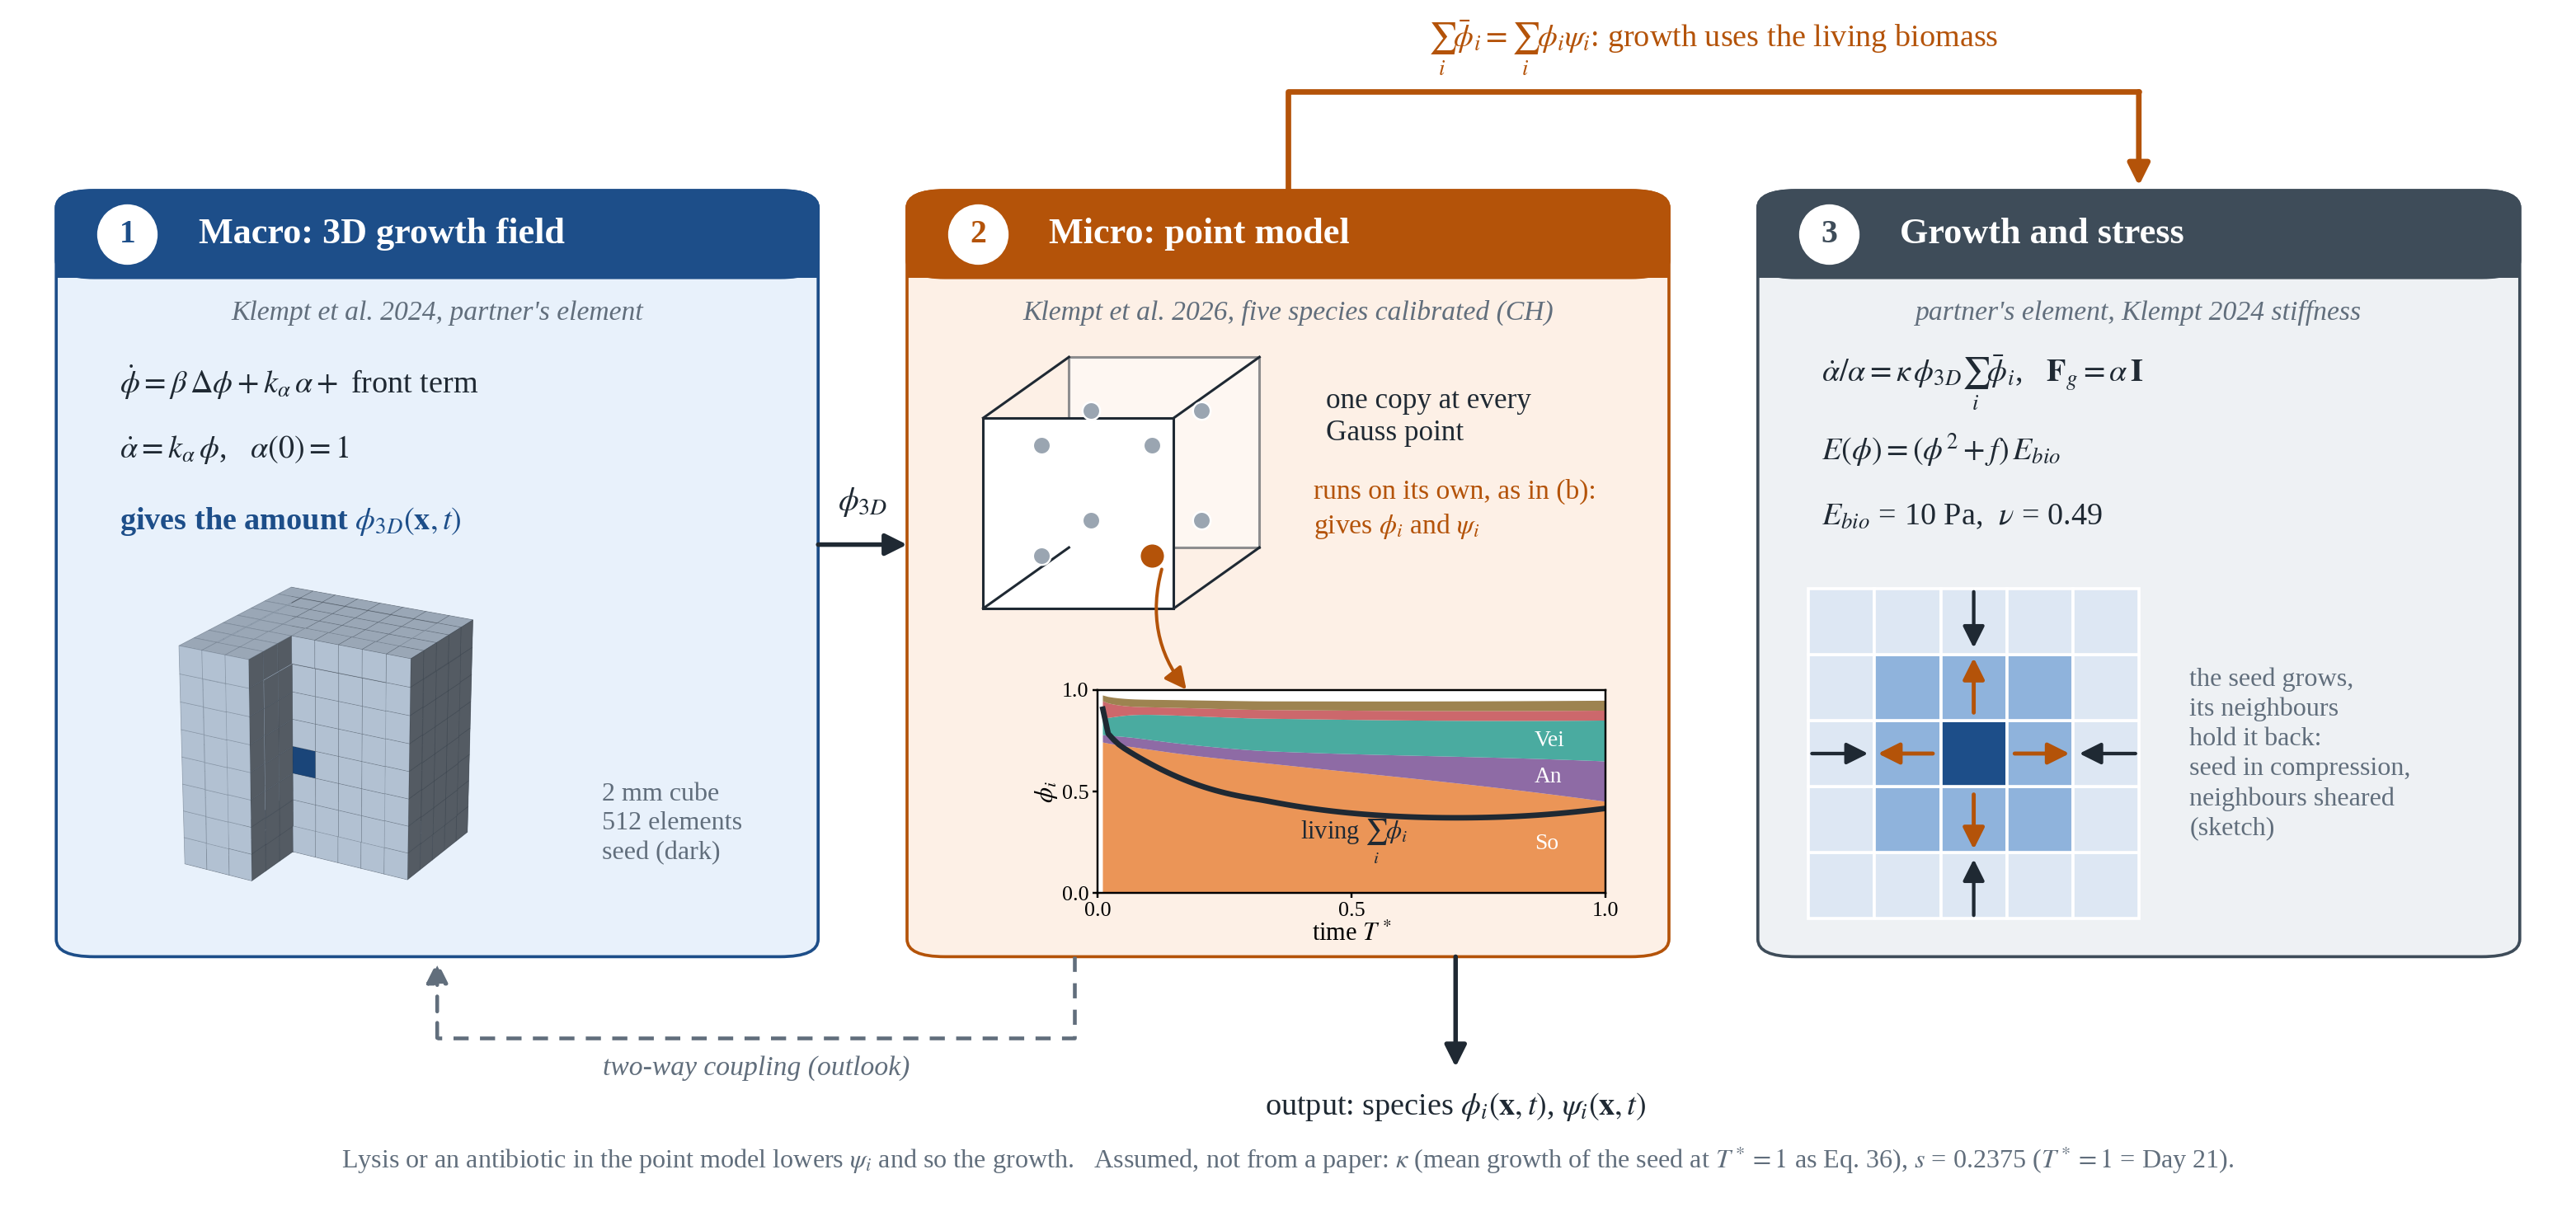
\includegraphics[width=\linewidth,height=0.5\textheight,keepaspectratio]{assets/fig_coupling_schematic_live.png}
\end{center}
\vspace{-8pt}
\begin{columns}[T]
\begin{column}{0.40\textwidth}
\scriptsize
Eq.\ 36 uses the amount: $\dot\alpha=k_\alpha\phi$.\\
Here: $\dot\alpha/\alpha=\kappa\,\phi_{3D}\sum_i\phi_i\psi_i$,
so lysis in the point model lowers the growth.\\[2pt]
$\kappa$ chosen so that the mean growth of the seed equals Eq.\ 36
(an assumption, not from a paper; Appendix E).
\end{column}
\begin{column}{0.58\textwidth}
\scriptsize\setlength\tabcolsep{2pt}
\begin{tabular}{@{}lrrr@{}}
\toprule
seed, $T^*=1$ & Eq.\ 36 & living & diff.\\
\midrule
$\alpha-1$, $8^3$ & $6.752\cdot10^{-4}$ & $6.752\cdot10^{-4}$ & $0.0\,\%$\\
von Mises$/E$, $8^3$ & $4.684\cdot10^{-5}$ & $4.357\cdot10^{-5}$ & $-7.0\,\%$\\
von Mises$/E$, $16^3$; $24^3$ & & & $-7.1$; $-7.0\,\%$\\
antibiotic vs.\ none, $8^3$ & $0\,\%$ & $-32\,\%$ & \\
\bottomrule
\end{tabular}\\[2pt]
five species calibrated (CH), $E=10$ Pa; the antibiotic
case with the previous calibration
\end{column}
\end{columns}
\end{frame}

% --------------------------------------------------------
\begin{frame}{Two modelling assumptions, each with a sensitivity study}
\begin{columns}[T]
\begin{column}{0.49\textwidth}
\centering\textbf{\small 1. time link $s=0.15$}\\[4pt]
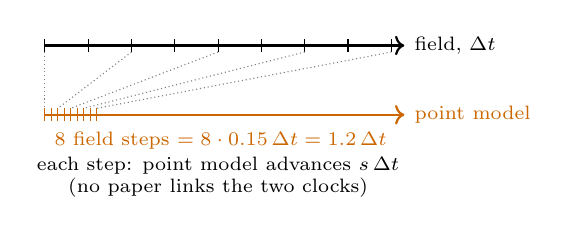
\begin{tikzpicture}[x=0.55cm,y=0.55cm]
\draw[thick,->] (0,1.6)--(8.3,1.6) node[right,font=\scriptsize]{field, $\Delta t$};
\foreach \k in {0,...,8} \draw (\k,1.45)--(\k,1.75);
\draw[thick,->,orange!80!black] (0,0)--(8.3,0) node[right,font=\scriptsize]{point model};
\foreach \k in {0,...,8} \draw[orange!80!black] (\k*0.15,-0.15)--(\k*0.15,0.15);
\foreach \k in {0,2,4,6,8} \draw[gray,densely dotted] (\k,1.45)--(\k*0.15,0.15);
\node[font=\scriptsize,orange!80!black,anchor=west] at (0,-0.6) {8 field steps $=8\cdot0.15\,\Delta t=1.2\,\Delta t$};
\node[font=\scriptsize,align=center] at (4,-1.45) {each step: point model advances $s\,\Delta t$\\(no paper links the two clocks)};
\end{tikzpicture}\\[6pt]
\scriptsize\renewcommand{\arraystretch}{1.15}
\begin{tabular}{@{}ll@{}}
\toprule
case (Klempt et al.\ 2026) & effect of $s$\\
\midrule
6: one species wins & winner appears for $s\gtrsim0.15$\\
3: coexistence & share moves by 0.03--0.06\\
\bottomrule
\end{tabular}
\end{column}
\begin{column}{0.49\textwidth}
\centering\textbf{\small 2. cap $\phi_{\rm cap}=0.9$}\\[4pt]
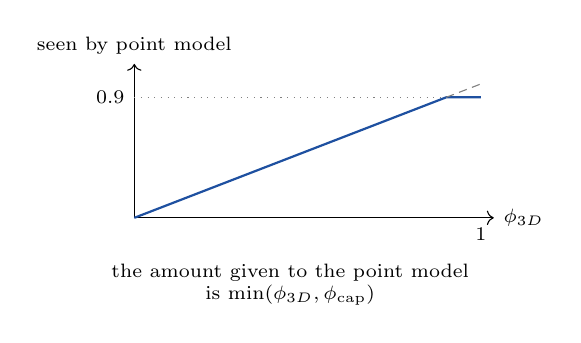
\begin{tikzpicture}[x=0.55cm,y=1.7cm]
\draw[->] (0,0)--(8.3,0) node[right,font=\scriptsize]{$\phi_{3D}$};
\draw[->] (0,0)--(0,1.15) node[above,font=\scriptsize]{seen by point model};
\draw[thick,c3] (0,0)--(7.2,0.9)--(8,0.9);
\draw[gray,densely dashed] (7.2,0.9)--(8,1.0);
\draw[gray,dotted] (0,0.9) node[left,font=\scriptsize,text=black]{0.9}--(7.2,0.9);
\node[font=\scriptsize] at (8,-0.12) {1};
\node[font=\scriptsize,align=center] at (3.6,-0.5) {the amount given to the point model\\is $\min(\phi_{3D},\phi_{\rm cap})$};
\end{tikzpicture}\\[6pt]
\scriptsize\renewcommand{\arraystretch}{1.15}
\begin{tabular}{@{}lccc@{}}
\toprule
$\phi_{\rm cap}$ & 0.85 & 0.90 & 0.95\\
\midrule
case 3 share & 0.668 & 0.667 & 0.664\\
\bottomrule
\end{tabular}
\end{column}
\end{columns}
\vspace{6pt}
\centering\small All other parameters are the published values.
\end{frame}

% --------------------------------------------------------
\begin{frame}{Limits}
\begin{columns}[T]
\begin{column}{0.48\textwidth}
\begin{itemize}
  \item composition is local, not carried with the front: effect on the mean
        $\le0.001$ (right, Python)
  \item $s$ has no source in a paper
  \item Eq.\ 34 as printed moves the colony instead of growing it (Appendix D)
  \item two $\alpha$: the element's own and Eq.\ 36 are integrated separately (Check 2)
\end{itemize}
\end{column}
\begin{column}{0.5\textwidth}
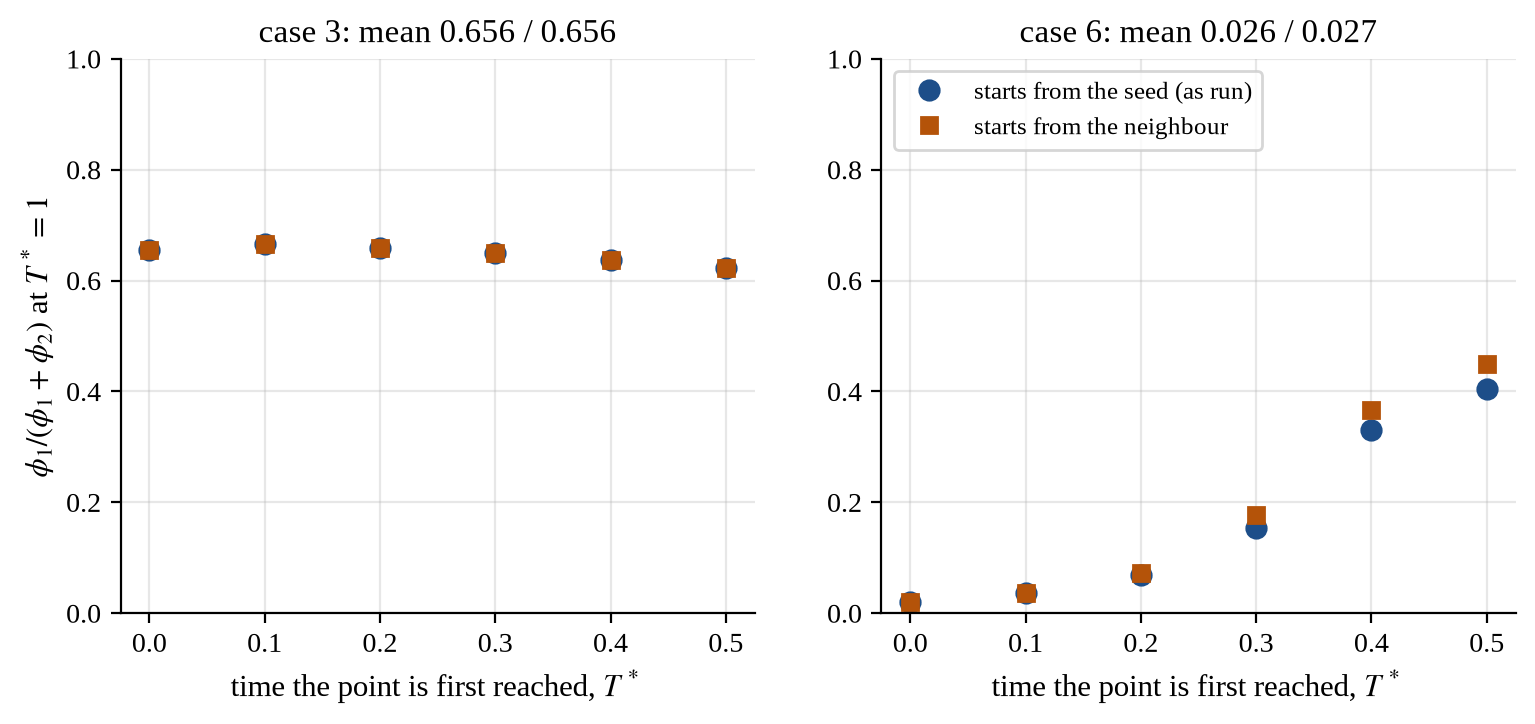
\includegraphics[width=\linewidth]{assets/fig_composition_transport_slide.png}\\
\scriptsize Composition at $T^*=1$ of the points first reached at each time; Klempt 2024
test case 4.1 field (Python, 20\,$\mu$m cube), Klempt 2026 cases 3 and 6.
\end{column}
\end{columns}
\end{frame}



% --------------------------------------------------------
\begin{frame}{Status and timeline}
\centering
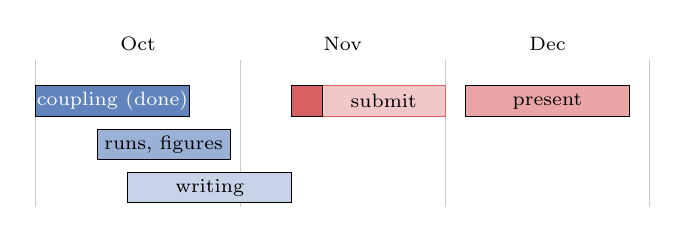
\begin{tikzpicture}[x=2.6cm, y=-0.55cm]
  \foreach \m/\lbl in {0/Oct, 1/Nov, 2/Dec} {
    \draw[gray!40] (\m,0) -- (\m,3.4);
    \node[above,font=\scriptsize] at (\m+0.5,0) {\lbl};
  }
  \draw[gray!40] (3,0) -- (3,3.4);
  \draw[fill=c3!70] (0,0.6) rectangle (0.75,1.3);
  \node[white,font=\scriptsize] at (0.375,0.95) {coupling (done)};
  \draw[fill=c3!45] (0.3,1.6) rectangle (0.95,2.3);
  \node[font=\scriptsize] at (0.625,1.95) {runs, figures};
  \draw[fill=c3!25] (0.45,2.6) rectangle (1.25,3.3);
  \node[font=\scriptsize] at (0.85,2.95) {writing};
  \draw[fill=warn!25,draw=warn!70] (1.25,0.6) rectangle (2.0,1.3);
  \draw[fill=warn!70] (1.25,0.6) rectangle (1.4,1.3);
  \node[font=\scriptsize] at (1.7,0.95) {submit};
  \draw[fill=warn!40] (2.1,0.6) rectangle (2.9,1.3);
  \node[font=\scriptsize] at (2.5,0.95) {present};
\end{tikzpicture}
\vspace{4pt}
\small
\begin{itemize}
  \item examiners Prof.\ Junker (IKM), Dr.\ Wangenheim (IDS); supervisors Dr.\ Soleimani, Dr.\ Geisler
  \item draft sent on 9 October; \textbf{submission 13 November}
  \item colloquium 16 December, 13:00, IKM room 320
  \item growth from the living biomass: not in the thesis, continued at Keio
\end{itemize}
\end{frame}

% --------------------------------------------------------
\begin{frame}{Questions for this meeting}
\begin{enumerate}
  \item \textbf{Your coupling ideas:} which direction would you take first?
  \item \textbf{Growth law:} amount of the field (Eq.\ 36) or living biomass of the point model?
  \item \textbf{Two-way coupling:} should the stress act back on the growth or the composition?
  \item \textbf{Rate $\kappa$:} fixed by the mean growth of Eq.\ 36, or by the measured volume?
  \item \textbf{Next steps:} what should be done here, and what at Keio?
\end{enumerate}
\end{frame}

% --------------------------------------------------------
\begin{frame}{References}
\small
\begin{itemize}
  \item Klempt, Soleimani, Junker (2023), PAMM: precursor spatial model
  \item Klempt, Soleimani, Wriggers, Junker (2024), Biomech.\ Model.\ Mechanobiol.:
        growth field, Eq.\ 34/36, Table 2
  \item Klempt, Geisler, Soleimani, Junker (2026), Arch.\ Appl.\ Mech.:
        multi-species point model, Table 1 cases
  \item Fritsch et al.\ (2025), arXiv:2512.15145: Bayesian updating, same model
\end{itemize}
\end{frame}


% ========================================================
% Appendix: notation and background
% ========================================================
\appendix
\begin{frame}{Appendix A: notation}
\scriptsize
\begin{columns}[T]
\begin{column}{0.5\textwidth}
\textbf{Growth field and mechanics (Klempt et al.\ 2024)}\\[2pt]
\begin{tabular}{@{}l>{\raggedright\arraybackslash}p{0.66\linewidth}@{}}
\toprule
$\phi$ & biofilm volume fraction (0 = void, 1 = dense)\\
$c$ & nutrient concentration\\
$\alpha$ & expansion variable, $\mathbf F_g=\alpha\mathbf I$, $\alpha(0)=1$; growth is $\alpha-1$\\
$\mathbf F=\mathbf F_e\mathbf F_g$ & elastic / growth split\\
$k_\alpha$ & growth factor ($10^{-3}$ per $T^*$)\\
$\beta$ & phase-field regularisation\\
$r,\ k$ & front growth rate, Monod constant\\
$T^*$ & normalised time, $T^*\in[0,1]$\\
\bottomrule
\end{tabular}
\end{column}
\begin{column}{0.48\textwidth}
\textbf{Point model (Klempt et al.\ 2026)}\\[2pt]
\begin{tabular}{@{}l>{\raggedright\arraybackslash}p{0.66\linewidth}@{}}
\toprule
$\phi_i$ & volume fraction of species $i$\\
$\phi_0$ & void, $\phi_0=1-\sum_i\phi_i$\\
$\psi_i$ & living fraction (viability) of species $i$\\
$\gamma$ & Lagrange multiplier for $\sum\phi_i+\phi_0=1$\\
$A_{ij}$ & interaction matrix (self, cooperation, competition)\\
$b_i$ & sensitivity to the antibiotic\\
$c^*,\ \alpha^*$ & nutrient, antibiotic concentration\\
$\eta_i$ & viscosity (time scale) of species $i$\\
\bottomrule
\end{tabular}\\[6pt]
\textbf{Coupling (this work)}\\[2pt]
\begin{tabular}{@{}l>{\raggedright\arraybackslash}p{0.66\linewidth}@{}}
\toprule
$\phi_{3D}$ & amount from the element field\\
$\phi_i/\sum_j\phi_j$ & composition (share of species $i$)\\
$s$ & time link: point model advances $s\,\Delta t$\\
$\phi_{\rm cap}$ & largest amount the point model sees\\
\bottomrule
\end{tabular}
\end{column}
\end{columns}
\end{frame}

% --------------------------------------------------------
\begin{frame}{Appendix B: background, growth field and mechanics}
\small
\textbf{Kinematics.} Growth is a volume change: $\mathbf F=\mathbf F_e\mathbf F_g$ with
isotropic $\mathbf F_g=\alpha\mathbf I$. Stress comes only from $\mathbf F_e$ (neo-Hookean).
A body that can grow freely stays stress free; stress appears where growth is constrained.\\
\textbf{Material} (Klempt et al.\ 2024, Eq.\ 20 and Table 2): $E=10$ Pa, $\nu=0.49$,
stiffness weighted with $\phi^2$ (void: floor $10^{-3}E$); no viscosity.
Stresses scale linearly with $E$ (the example input's 1000 MPa gives $10^8\times$ larger values).
\vspace{4pt}

\textbf{Field equations} (Klempt et al.\ 2024, from an extended Hamilton principle):
\[
\dot\phi=\underbrace{\beta\,\Delta\phi}_{\text{diffusion}}
+\underbrace{k_\alpha\,\alpha}_{\text{local source}}
-\underbrace{r\,\frac{c}{k+c}\,\nabla\phi\cdot\frac{\nabla c}{|\nabla c|}}_{\text{front growth towards nutrient}},
\qquad
\dot\alpha=k_\alpha\,\phi
\]
\begin{itemize}
  \item $\phi$ and $c$ are nodal fields of the element; $\alpha$ is an internal
        variable at the Gauss points
  \item The front term moves the biofilm boundary up the nutrient gradient; it vanishes
        where $\phi$ or $c$ is uniform
  \item The nutrient diffuses much faster than the biofilm grows (quasi-static $c$)
\end{itemize}
\end{frame}

% --------------------------------------------------------
\begin{frame}{Appendix C: point model and one substep of the coupled run}
\footnotesize
\textbf{Point model} (Klempt et al.\ 2026), per species $i$, no space dependence, implicit, $\Delta t=10^{-4}$:
\vspace{-4pt}
\[
\begin{aligned}
(\eta_{\phi,i}+\eta_i\psi_i^2)\,\dot\phi_i+\eta_i\phi_i\psi_i\,\dot\psi_i
&= c^*\psi_i\textstyle\sum_j A_{ij}\phi_j\psi_j-\gamma-(\text{barrier})\\[-2pt]
\eta_i\,(\phi_i\psi_i\,\dot\phi_i+\phi_i^2\,\dot\psi_i)
&= c^*\phi_i\textstyle\sum_j A_{ij}\phi_j\psi_j-\alpha^* b_i\,\psi_i-(\text{barrier}),
\qquad \textstyle\sum_i\phi_i+\phi_0=1
\end{aligned}
\]
\vspace{-6pt}

\textbf{One substep $t_n\to t_{n+1}$}: ANSYS solves only $\operatorname{div}\boldsymbol\sigma=\mathbf 0$;
the material routine turns $\mathbf F$ into $\boldsymbol\sigma$ after removing the growth.\\[2pt]
\scriptsize
\renewcommand{\arraystretch}{1.0}
\begin{tabular}{@{}r@{\hspace{6pt}}l@{}}
\textcolor{gray}{1} & \textbf{repeat} \textcolor{gray}{(Newton iteration of ANSYS)}\\
\textcolor{gray}{2} & \quad $\mathbf F$ at every Gauss point from the current displacements\\
\textcolor{gray}{3} & \quad \textbf{for each Gauss point}\\
\textcolor{gray}{4} & \quad\quad $\phi_{3D}=\phi_1+\phi_2$ from the element; restore the converged state of $t_n$\\
\textcolor{gray}{5} & \quad\quad $\alpha_{n+1}=\alpha_n+k_\alpha\,\phi_{3D}\,\Delta t$ \hfill\textcolor{gray}{Eq.\ 36}\\
\textcolor{gray}{6} & \quad\quad $\mathbf F_e=\mathbf F\,\mathbf F_g^{-1}$, $\mathbf F_g=\alpha_{n+1}\mathbf I$ $\;\to\;$ $\boldsymbol\sigma$, tangent\\
\textcolor{gray}{7} & \quad\quad \textbf{if} two species and $\phi_{3D}\ge\phi_{\min}$:\\
\textcolor{gray}{8} & \quad\quad\quad scale the point model to $\min(\phi_{3D},\phi_{\rm cap})$\\
\textcolor{gray}{9} & \quad\quad\quad bridge (Fortran $\to$ C $\to$ socket $\to$ Python): $n_{\rm sub}$ steps of $s\Delta t/n_{\rm sub}$\\
\textcolor{gray}{10} & \quad\quad\quad scale back; store $\phi_i,\psi_i,\gamma$ as state variables\\
\textcolor{gray}{11} & \quad\quad return $\boldsymbol\sigma$ and the tangent to ANSYS\\
\textcolor{gray}{12} & \quad assemble the residual, update the displacements\\
\textcolor{gray}{13} & \textbf{until} converged\\
\textcolor{gray}{14} & the element advances $\phi_1,\phi_2,c$ to $t_{n+1}$ (its own solver)\\
\end{tabular}
\end{frame}

% --------------------------------------------------------
\begin{frame}{Appendix D: Klempt et al.\ 2024 test cases, reproduced in Python}
\vspace{-6pt}
\begin{center}
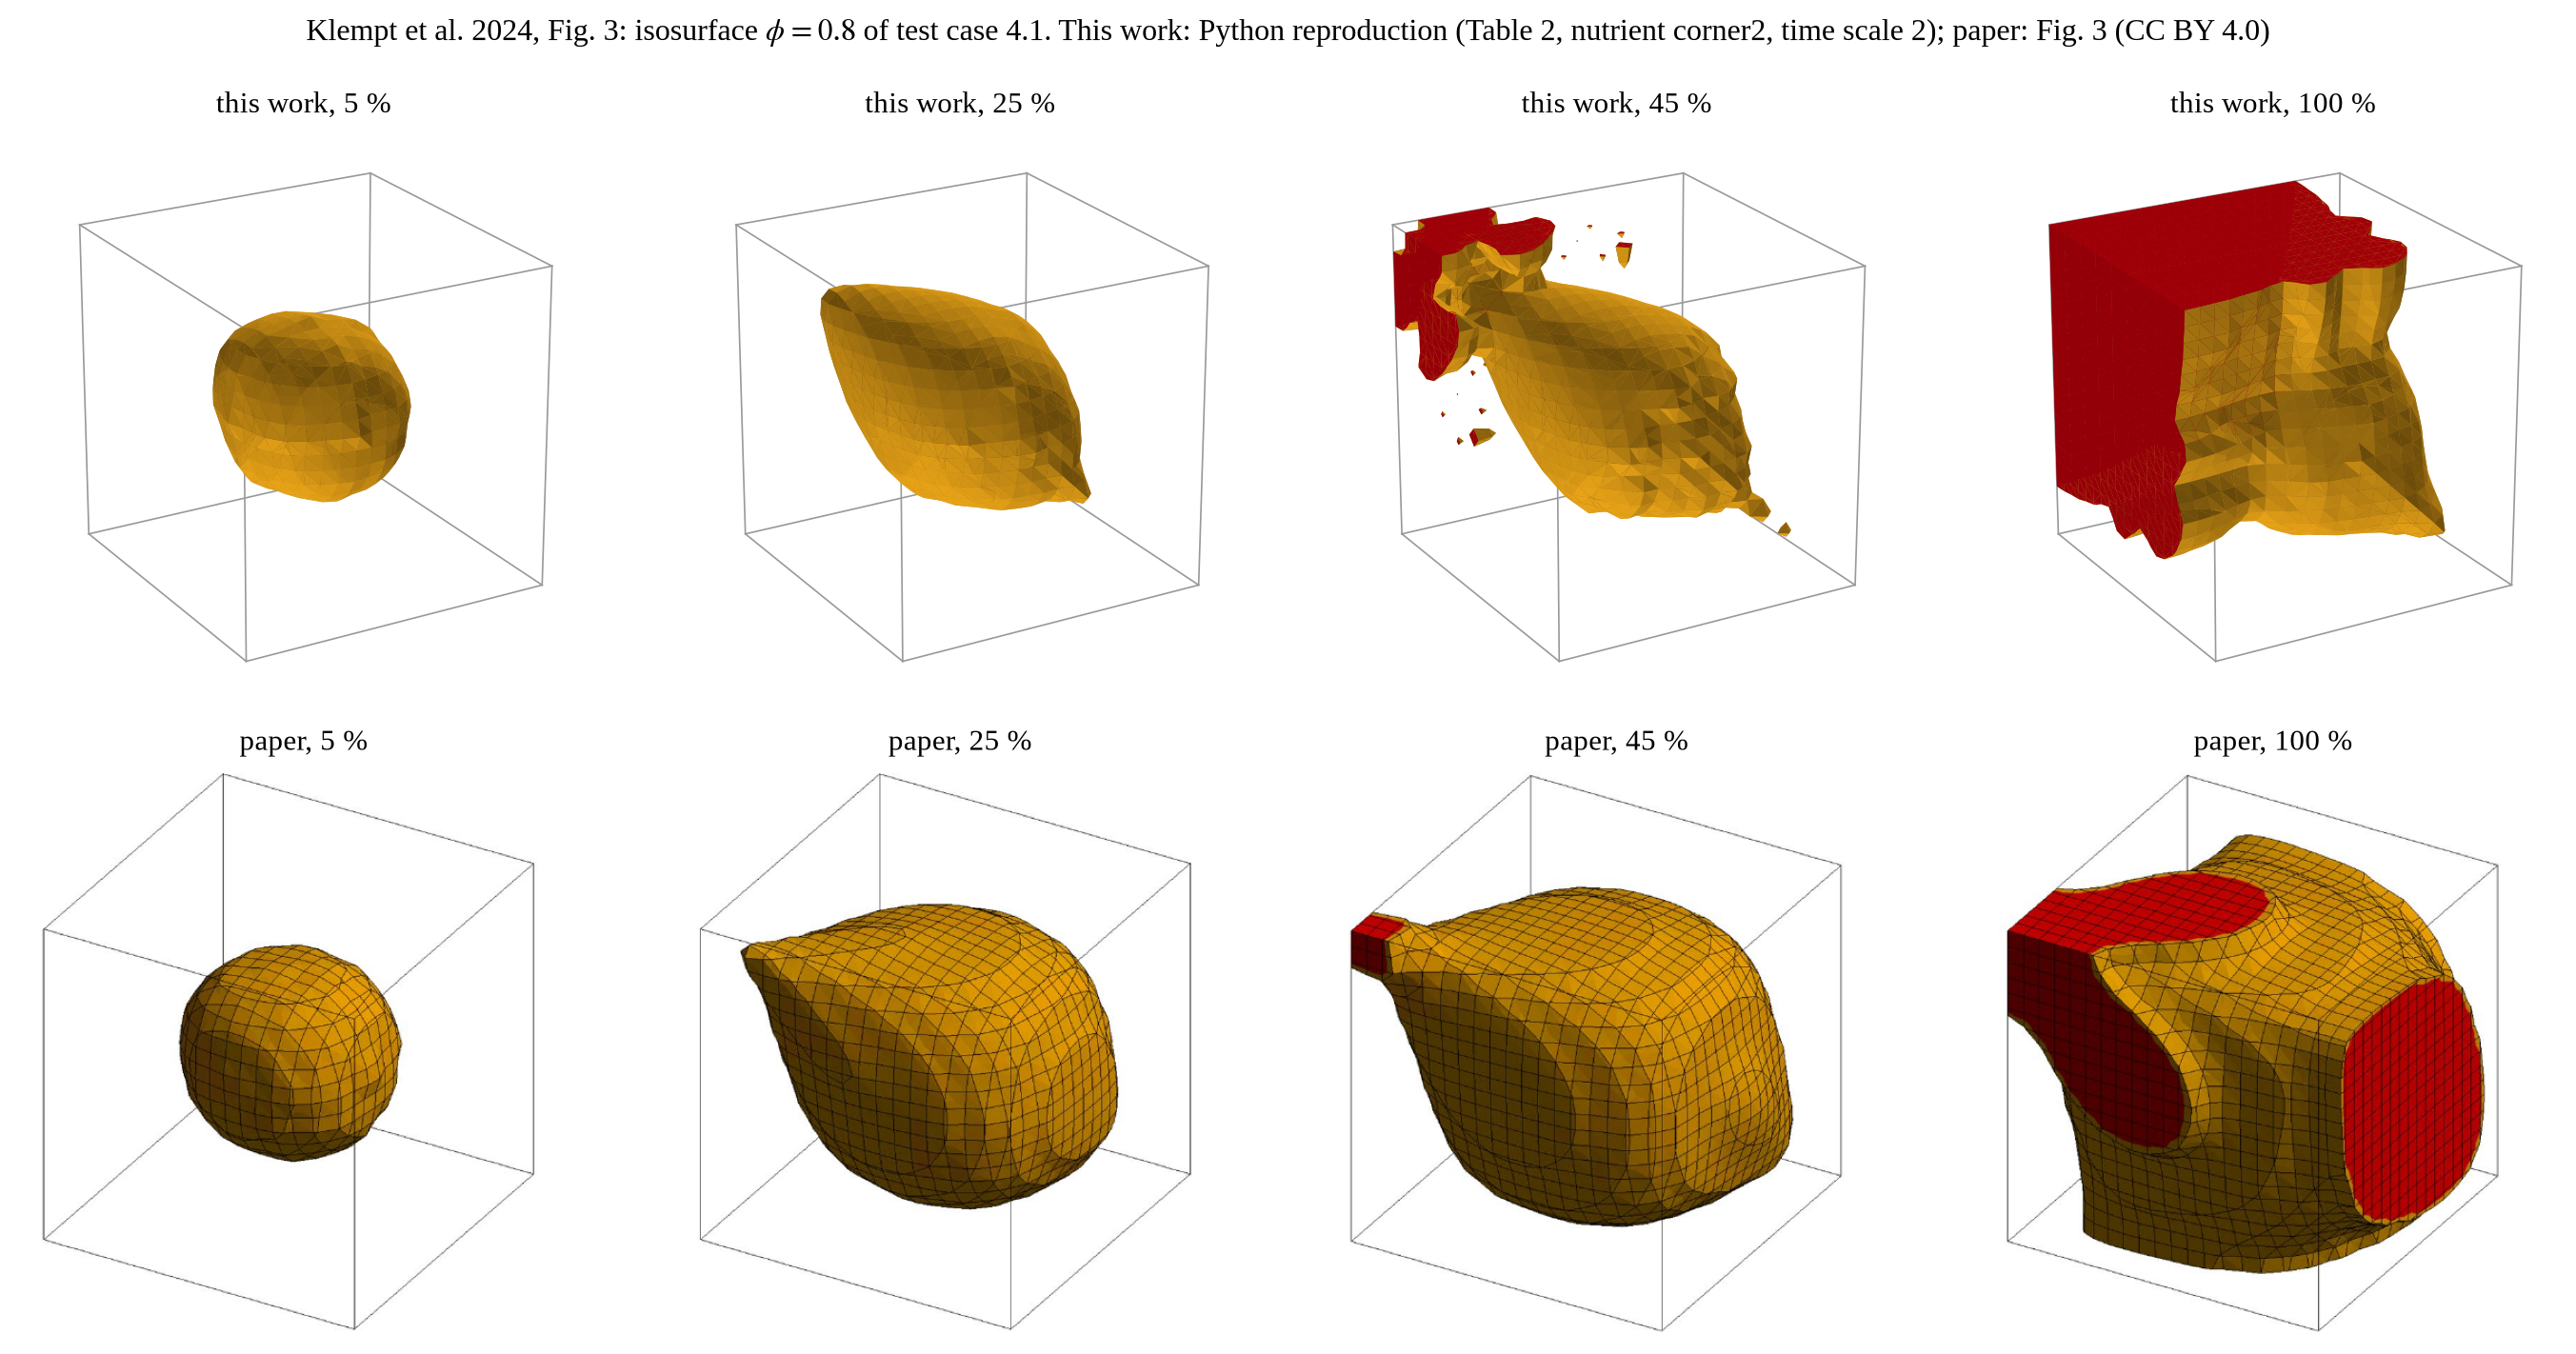
\includegraphics[width=\linewidth,height=0.47\textheight,keepaspectratio]{assets/fig_klempt2024_fig3.png}
\end{center}
\vspace{-8pt}
\scriptsize
\begin{columns}[T]
\begin{column}{0.47\textwidth}
\begin{tabular}{@{}lccc@{}}
\toprule
test case & time scale & RMS $\phi$ & RMS $c$\\
\midrule
4.1 (Fig.\ 4) & 2 & 0.03 & 0.02\\
4.2 ``high'' (Fig.\ 7) & 10 & 0.04 & 0.04\\
4.2 ``low'' (Fig.\ 7) & 4--5 & 0.09 & 0.05\\
\bottomrule
\end{tabular}
\end{column}
\begin{column}{0.51\textwidth}
Independent solver on the paper's 20\,$\mu$m cube, not the ANSYS model.
Table 2 unchanged; growth on both faces and consumption $g\phi c$ (two
departures from Eq.\ 34/35 as printed); nutrient in a 2\,$\mu$m corner block;
one time scale per run ($T^*=t/t_{\rm ref}$, Sec.\ 4). Curves agree; the
shape agrees in kind (egg towards the corner) but is more slender, also with
other diffusion and a 2nd-order scheme. Table 3's pressure fits $\mu$ in MPa.
\end{column}
\end{columns}
\end{frame}

% --------------------------------------------------------
\begin{frame}{Appendix E: growth from the living biomass, implementation and runs}
\vspace{-6pt}
\[
\ln\alpha_{n+1}=\ln\alpha_n+\kappa\,\phi_{3D}\!\int_{t_n}^{t_{n+1}}\!\sum_i\phi_i\psi_i\,dt
\qquad\text{(Appendix C, line 5 only)}
\]
\vspace{-4pt}
\begin{columns}[T]
\begin{column}{0.42\textwidth}
\scriptsize\renewcommand{\arraystretch}{1.15}
\begin{tabular}{@{}>{\raggedright}p{0.3\linewidth}>{\raggedright\arraybackslash}p{0.66\linewidth}@{}}
\toprule
item & how\\
\midrule
form & increment of $\ln\alpha$, as Klempt 2024 Table 1\\
$\phi_{3D}\in[0,1]$ & only marks where the biofilm is\\
point model & one per Gauss point, on its own (not scaled to $\phi_{3D}$)\\
start & when $\phi_{3D}\ge\phi_{\min}$, from the calibrated Day-1 state\\
integral & over its own substeps, clock $s$ per unit $T^*$\\
storage & state variables of the Gauss point; element unchanged\\
$\kappa$ & $8.14\cdot10^{-3}$: mean $\alpha-1$ as Eq.\ 36 ($-0.003\,\%$); assumed\\
\bottomrule
\end{tabular}
\end{column}
\begin{column}{0.54\textwidth}
\scriptsize\setlength\tabcolsep{2pt}\renewcommand{\arraystretch}{1.15}
\begin{tabular}{@{}lrrr@{}}
\toprule
seed, $T^*=1$ & Eq.\ 36 & living & diff.\\
\midrule
$\alpha-1$, $8^3$ & $6.752\cdot10^{-4}$ & $6.752\cdot10^{-4}$ & $0.0\,\%$\\
von Mises$/E$, $8^3$ & $4.684\cdot10^{-5}$ & $4.357\cdot10^{-5}$ & $-7.0\,\%$\\
vM, $16^3$; $24^3$ & & & $-7.1$; $-7.0\,\%$\\
vM$/(E(\alpha-1))$ & $0.069$ & $0.064$ & \\
antibiotic, $8^3$ & $0\,\%$ & $-32\,\%$ & \\
\bottomrule
\end{tabular}\\[3pt]
CH, $E=10$ Pa, $\nu=0.49$; the antibiotic case with the previous calibration.
Same amount of growth, different spread inside the seed; $\alpha-1$ and stress scale with $\kappa$.
\end{column}
\end{columns}
\end{frame}

% --------------------------------------------------------
\begin{frame}{Appendix F: how the run is implemented, and the tools}
\vspace{-4pt}
\begin{center}
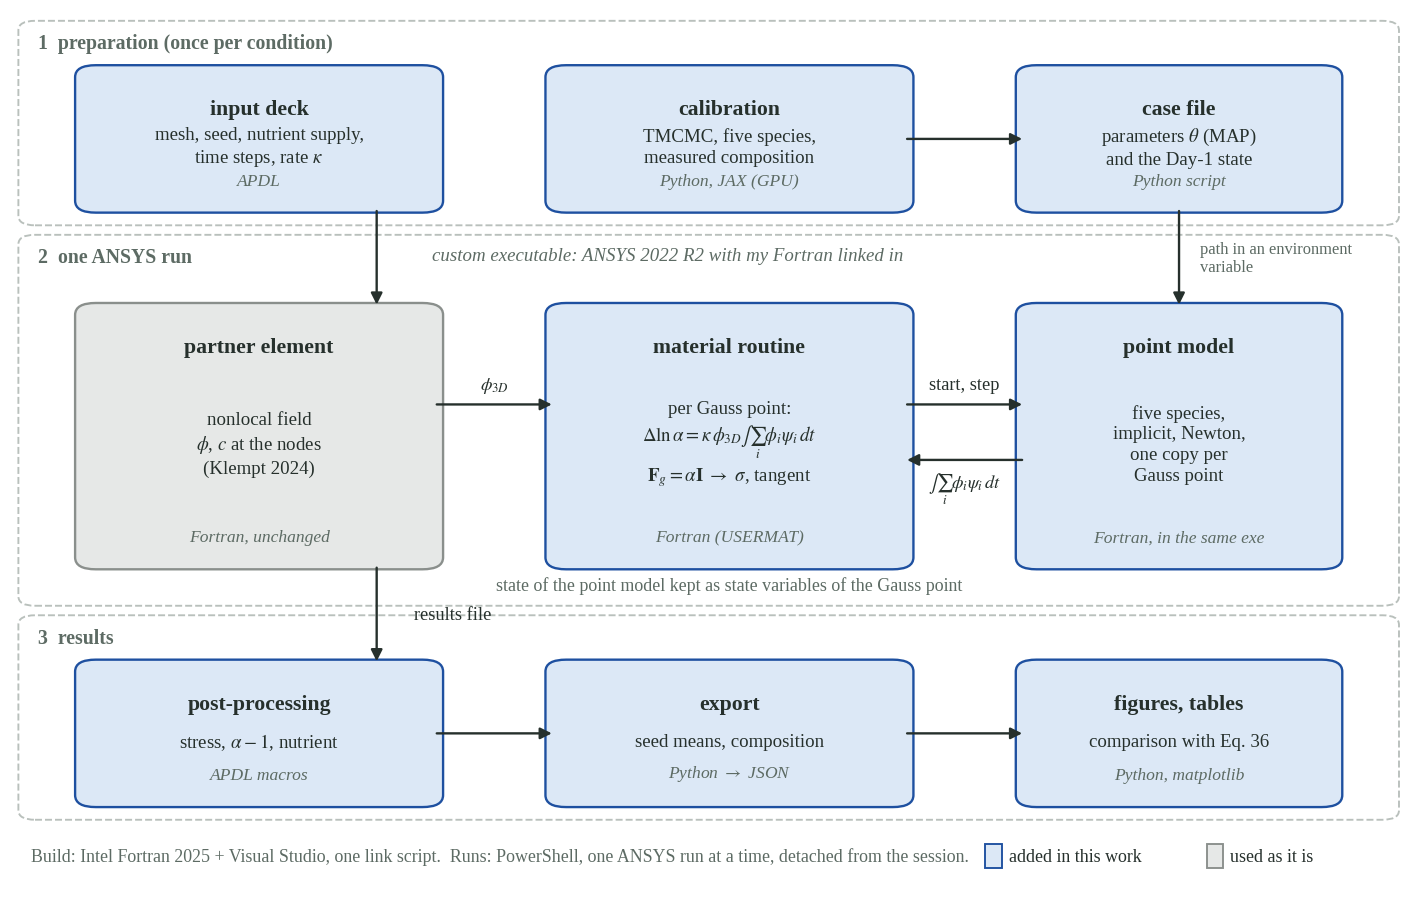
\includegraphics[width=\linewidth,height=0.8\textheight,keepaspectratio]{assets/fig_implementation_tools.png}
\end{center}
\vspace{-6pt}
\scriptsize Blue: added in this work; grey: used as it is. One line of the material routine changes
compared with Eq.\ 36.
\end{frame}

% --------------------------------------------------------
\begin{frame}{Appendix G: calibrated five-species model in the element}
\vspace{-4pt}
\begin{center}
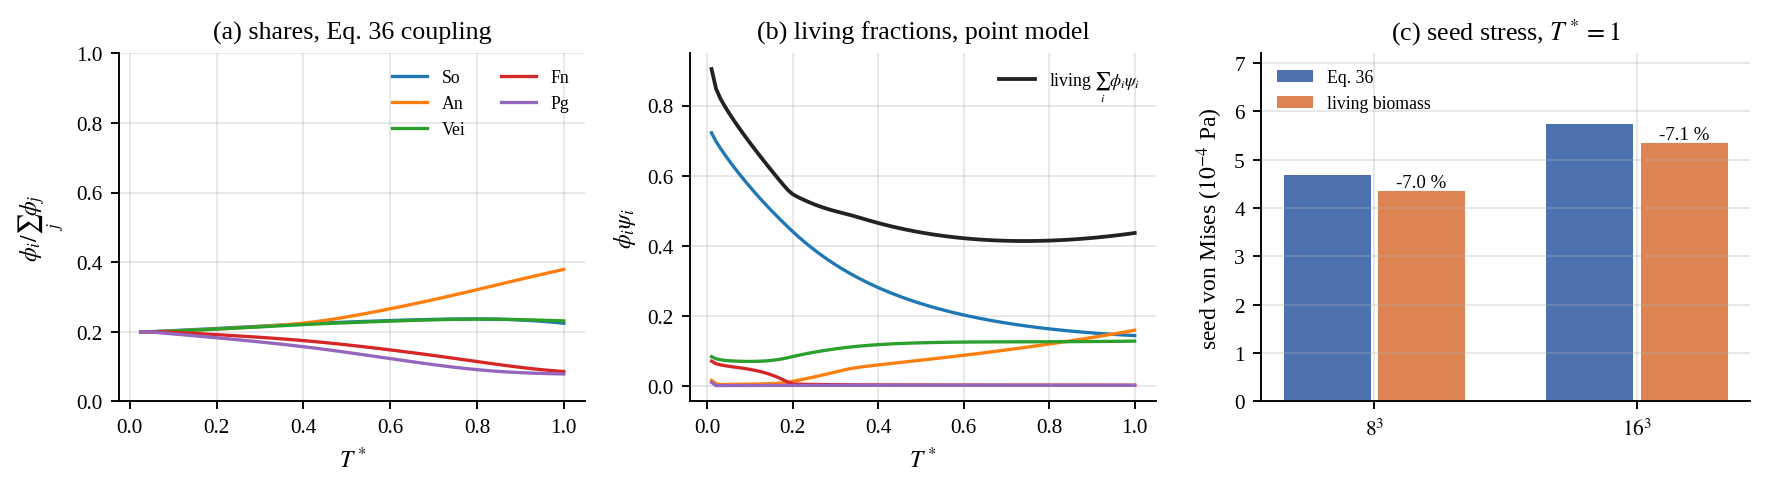
\includegraphics[width=\linewidth]{assets/fig_cal5_appendix.png}
\end{center}
\vspace{-4pt}
\scriptsize\renewcommand{\arraystretch}{1.15}\setlength\tabcolsep{3pt}
\begin{tabular}{@{}>{\raggedright}p{0.15\linewidth}>{\raggedright}p{0.07\linewidth}>{\raggedright}p{0.27\linewidth}>{\raggedright}p{0.19\linewidth}>{\raggedright\arraybackslash}p{0.24\linewidth}@{}}
\toprule
 & start & $T^*=1$ & growth $\alpha-1$ & seed von Mises\\
\midrule
shares (Eq.\ 36) & 0.2 each & An 0.38, Vei 0.23, So 0.23, Fn 0.09, Pg 0.08 & $6.752\cdot10^{-4}$, same as two species & vM$/E=4.68\cdot10^{-5}$\\
living biomass $\sum_i\phi_i\psi_i$ & 0.90 & 0.44 (mostly So lost) & same mean & $-7.0\,\%$ ($8^3$),\newline $-7.1\,\%$ ($16^3$)\\
\bottomrule
\end{tabular}\\[3pt]
commensal flow condition (CH), calibration to the measured data, $E=10$ Pa, $8^3$
\end{frame}

% --------------------------------------------------------
\begin{frame}{Appendix H: two and five species, implementation}
\footnotesize
\renewcommand{\arraystretch}{1.2}
\begin{tabular}{@{}>{\raggedright}p{0.17\linewidth}>{\raggedright}p{0.38\linewidth}>{\raggedright\arraybackslash}p{0.39\linewidth}@{}}
\toprule
 & two species (5 October) & five species (since 10 October)\\
\midrule
point model & Python, through a material server (Fortran $\to$ C $\to$ socket $\to$ Python) &
  Fortran, in the same executable (no server, about 4 times faster, same results)\\
parameters & Klempt et al.\ 2026 cases 3 and 6 ($c^*=100$, $\alpha^*=10$) &
  calibration (TMCMC, MAP, $5\times5$ interactions), $c^*=25$, $\alpha^*=0$\\
start & equal shares & equal shares; calibrated Day-1 state for the living-biomass growth\\
stiffness & partner's example input, $E=1000$ MPa & Klempt 2024, $E=10$ Pa\\
coupling (Eq.\ 36) & \multicolumn{2}{l}{same code: amount scaled to $\phi_{3D}$, $\phi_{\rm cap}=0.9$, time link $s=0.15$}\\
growth from the living biomass & -- & yes; point model runs on its own, $s=0.2375$ ($T^*=1$ is Day 21)\\
\bottomrule
\end{tabular}\\[6pt]
\footnotesize The number of species is a parameter (1 to 5) of the same routine.
\end{frame}

% --------------------------------------------------------
\begin{frame}{Appendix I: fields on the mid-plane over time}
\vspace{-6pt}
\begin{center}
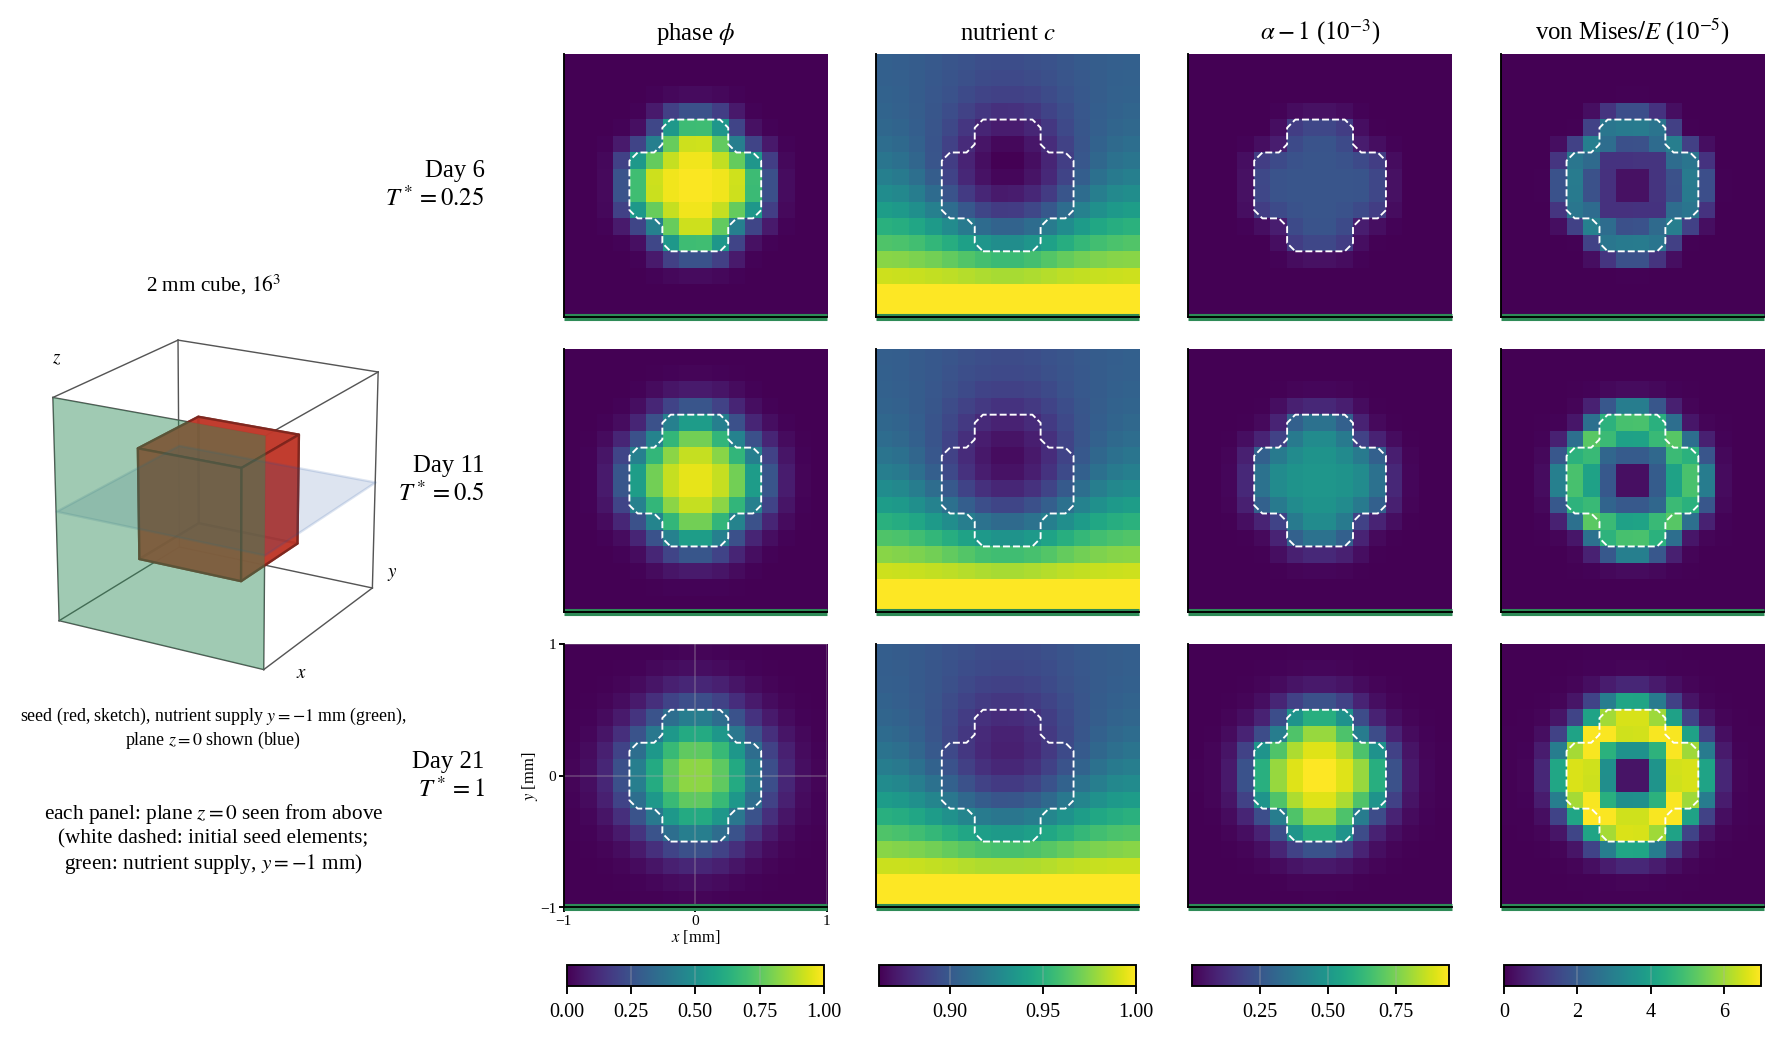
\includegraphics[width=\linewidth,height=0.8\textheight,keepaspectratio]{assets/fig_fields_time.png}
\end{center}
\vspace{-8pt}
\scriptsize Plane $z=0$ seen from above ($x$ right, $y$ up), $16^3$, CH calibrated to the measured data.
Growth by Eq.\ 36. The phase spreads and thins, the nutrient is used around the seed, and the stress forms a ring at the seed edge.
\end{frame}

% --------------------------------------------------------
\begin{frame}{Appendix J: analysis conditions}
\scriptsize\renewcommand{\arraystretch}{1.15}
\begin{tabular}{@{}>{\raggedright}p{0.2\linewidth}>{\raggedright\arraybackslash}p{0.76\linewidth}@{}}
\toprule
geometry, mesh & 2 mm cube; $8^3$ (512), $16^3$, $24^3$ hexahedral elements; seed of 32 elements at the centre ($8^3$, refined with the mesh)\\
mechanical BC & only rigid-body motion fixed (corner nodes); otherwise traction free\\
nutrient BC & $c=1$ on the face $y=-1$ mm; no flux elsewhere\\
initial state & $\phi=1$ in the seed, $\approx0$ outside; $\alpha=1$; $c=1$ everywhere\\
time & $T^*=1$ is Day 21; $\Delta T^*=0.025$ (40 steps; living-biomass runs: $1/95$); ANSYS 2022 R2, static, nonlinear geometry\\
material & neo-Hooke, $E=10$ Pa, $\nu=0.49$, $E\propto\phi^2$ (Klempt 2024 Table 2); $\mathbf F_g=\alpha\mathbf I$\\
growth field & $k_\alpha=10^{-3}$, $\beta=0.02$ mm$^2/T^*$ (Table 2 scaled to the 2 mm cube, assumed)\\
point model & two species: Klempt 2026 cases 3 and 6; five species: calibrated MAP (CH), $c^*=25$\\
coupling & $\phi_{\rm cap}=0.9$, $\phi_{\min}=0.01$, time link $s=0.15$ (assumed);
            living-biomass growth: $s=0.2375$, $\kappa=8.14\cdot10^{-3}$ (assumed)\\
output & seed means of $\alpha-1$ and von Mises$/E$ at $T^*=1$\\
\bottomrule
\end{tabular}\\[4pt]
Values not from a paper are marked as assumed.
\end{frame}

% --------------------------------------------------------
\begin{frame}{Appendix K: mesh convergence}
\vspace{-4pt}
\begin{center}
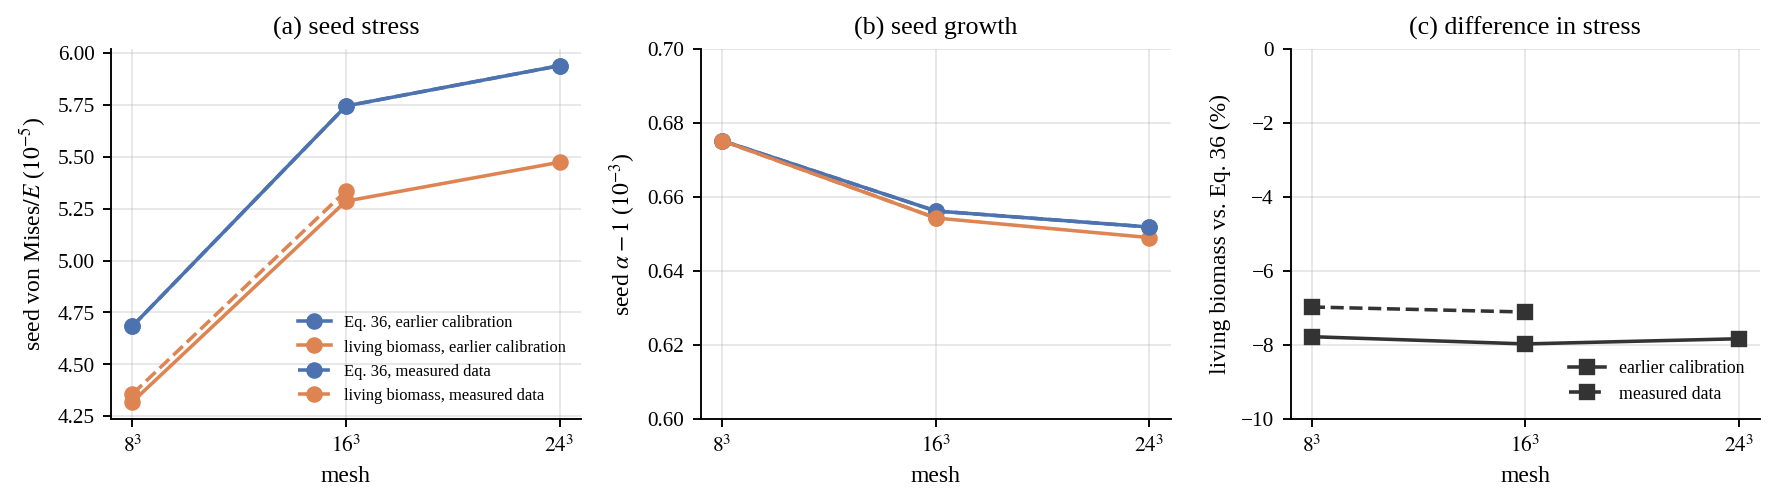
\includegraphics[width=\linewidth,height=0.42\textheight,keepaspectratio]{assets/fig_mesh_convergence.png}
\end{center}
\vspace{-6pt}
\scriptsize\setlength\tabcolsep{4pt}
\begin{tabular}{@{}lrrrr@{}}
\toprule
mesh & elements & nodes & integration points & seed elements\\
\midrule
$8^3$ & 512 & 729 & 4\,096 & 32\\
$16^3$ & 4\,096 & 4\,913 & 32\,768 & 256\\
$24^3$ & 13\,824 & 15\,625 & 110\,592 & 864\\
\bottomrule
\end{tabular}
\hfill
\begin{minipage}[t]{0.42\linewidth}\vspace{-30pt}
\begin{itemize}
  \item seed stress: $+23\,\%$ from $8^3$ to $16^3$, $+3.4\,\%$ from $16^3$ to $24^3$; converging
  \item seed growth changes by less than $3.5\,\%$
  \item difference of the growth laws: $-7$ to $-8\,\%$ on every mesh
  \item measured-data calibration: $-7.0\,\%$ at $8^3$ and $24^3$, $-7.1\,\%$ at $16^3$
\end{itemize}
\end{minipage}\\[2pt]
8 integration points per hexahedral element ($2\times2\times2$)
\end{frame}

% --------------------------------------------------------
\begin{frame}{Appendix L: finite element formulation}
\scriptsize\renewcommand{\arraystretch}{1.15}
\begin{tabular}{@{}>{\raggedright}p{0.2\linewidth}>{\raggedright\arraybackslash}p{0.76\linewidth}@{}}
\toprule
balance & $\operatorname{div}\boldsymbol\sigma=\mathbf 0$ in the current configuration, no body force; weak form by ANSYS (static, large deformation)\\
kinematics & $\mathbf F=\mathbf F_e\mathbf F_g$, $\mathbf F_g=\alpha\mathbf I$; Cauchy stress from $\mathbf F_e$\\
material & neo-Hooke in $\mathbf F_e$, stiffness $(\phi^2+f)E$ with a small void part $f$; tangent returned by the material routine\\
element & SOLID185, 8 nodes, $2\times2\times2$ integration with B-bar (default), for $\nu=0.49$\\
nonlinear solver & full Newton--Raphson, fixed steps (no automatic time stepping), up to 50 iterations, default force tolerance\\
coupling & staggered: ANSYS solves the mechanics with $\phi$ fixed; at the end of each step the partner element
            updates $\phi$ explicitly and solves the nutrient (linear system, PARDISO) on its neighbour operator\\
stability & explicit update of $\phi$: $\Delta t\le h^2/(2\beta)$; met for all meshes used\\
supports & 3-2-1: one corner node $u_x,u_y,u_z$, one $u_y,u_z$, one $u_z$ (6 dofs, only rigid-body motion)\\
\bottomrule
\end{tabular}\\[6pt]
\textbf{Time step} (one species, $8^3$, $T^*=1.1$): $\Delta T^*=0.1\to0.05\to0.025$ changes the seed von Mises$/E$ by
$-3.0\,\%$ and $-1.5\,\%$ ($\alpha-1$: $-0.7\,\%$, $-0.3\,\%$), first order; the runs use $\Delta T^*=0.025$, the living-biomass runs $1/95\approx0.011$.
\end{frame}

\end{document}
